\normalsize
\section{Standing Wave Test}
\label{chapter:NumericalTest-StaWav}

The standing wave motion in a closed basin is used to evaluate the free-surface non-hydrostatic numerical model. The analytical solution for such case can be approximated by the small amplitude wave theory as documented in the Appendices of \cite{LeBlond1978} and \cite{Jankowski1999}. Several assumptions are made in this theory: the fluid is inviscid, incompressible, with constant density and negligible surface tension; the depth of the fluid is uniform when in equilibrium; the nonlinear terms in the momentum equations are negligible. Therefore the governing equation can be written as
\be
\f{\p u_i}{\p t} =-\f{1}{\rho}\f{\p p}{\p x_i} \label{eqn:chap-test-momentum-Small-Amplitude-Wave}
\ee
\be
p=-\rho g (\eta-z) +p_d = p_o + \rho g \eta +p_d = p_o + p'
\ee
where $\eta$ is the surface position, $p_o$ is the equilibrium pressure, $p_d$ is the hydrodynamic/non-hydrostatic pressure, and $p'$ is the perturbation pressure. Plugging in this momentum equation into the continuity equation,
\be
\f{\p u_i}{\p x_i}=0
\ee
gives the pressure Poisson equation,
\be
\f{\p^2 p}{\p x_i^2}=0
\ee
or
\be
\f{\p^2 p'}{\p x_i^2}=0
\ee


For the surface distribution of the sinusoidal form with amplitude $A$,
\be
\eta = A \cos(k_x x+k_y y -\omega t)
\ee
the perturbation pressure $p'$ is assumed to be proportional to this surface distribution, hence the pressure Poisson equation becomes
\be
\f{\p p'}{\p z^2}-(k_x^2 + k_y^2) p' = 0
\ee
With the top ($z=\eta$) and bottom (at the equilibrium depth $z=-d$) boundary conditions,
\be
p'|_{z=\eta} = \rho g \eta,   \hspace{0.5in}  \left.\f{\p p'}{\p z }\right|_{z=-d} = 0
\ee
one solution can be found as
\be
p'= \rho g A \f{\cosh[k(z+d)]}{\cosh(kd)}\cos(k_x x +k_y y -\omega t)
\ee
where $k^2=k_x^2+k_y^2$ is the wave number. From the simplified momentum equation, the velocity can be derived,
\be
u= g A \f{k_x}{\omega} \frac{\cosh[k(z+d)]}{\cosh(kd)}\cos(k_x x+k_y y - \omega t)
\ee
\be
v= g A \f{k_y}{\omega} \frac{\cosh[k(z+d)]}{\cosh(kd)}\cos(k_x x+k_y y - \omega t)
\ee
\be
w= g A \f{k}{\omega} \frac{\cosh[k(z+d)]}{\cosh(kd)}\cos(k_x x+k_y y - \omega t)
\ee

The kinematic boundary condition at the surface,
\be
\f{\p \eta}{\p t}+u \f{\p \eta}{\p x}+v \f{\p \eta}{\p y} - w =0
\ee
is simplified by neglecting the two terms involve the slope of the free surface,
\be
\f{\p \eta}{\p t} - w =0
\ee
hence the dispersion relation can be found as
\be
\omega^2 =gk \tanh(kd)
\ee

For two-dimensional case ($k_y=0$), the equation for standing waves with the small amplitude assumptions can be written as:
\begin{equation}
\eta = A \cos(kx)\cos(\omega t)
\end{equation}
\begin{equation}
u=\omega A \frac{\cosh[k(z+d)]}{\sinh(kd)}\sin(kx)\sin(\omega t)
\end{equation}
\begin{equation}
w=-\omega A \frac{\sinh[k(z+d)]}{\sinh(kd)}\cos(kx)\sin(\omega t)
\end{equation}
\begin{equation}
C= \omega /k
\end{equation}
\begin{equation}
k=2 \pi/L
\end{equation}
\begin{equation}
\omega^2=gk \tanh(kd)
\end{equation}
where $L$ is the length of the container. In the numerical test, the length of the container is set to be $L=10(m)$;
the equilibrium water depth is $d=10(m)$; the wave amplitude is
$A=0.1(m)$; the initial free surface is specified as $\eta_0 = A
cos(kx)$. Therefore the celerity of the wave can be derived as $C= \sqrt{\frac{gL}{2
\pi}tanh \frac{2 \pi h}{L}}=5.575 (m/s)$; and the period of the
oscillation is: $ T=2L/C= 3.587 (s)$.

Several grid resolutions are first tested in the numerical model: $20 \times 20$, $40 \times 40$, $80 \times 80$, and a three-dimensional case of $20(NX) \times 20(NZ) \times 10(NY)$. The computational time steps are fixed for each grid resolution. They are chosen to be the largest factors of one-eighth of the oscillation period ($T/8$) that can stably finish the simulation time of that complete oscillation period ($T$).

For the test case with resolution $20 \times 20$ and time step $\Delta t = 0.44845 (sec)$, the numerical results of velocity and hydrodynamic pressure at $t=1/8T$, $t=1/2T$ , and $t=5/8T$ are shown along with the analytical solutions in Figure \ref{fig:StanWav-1-8}, \ref{fig:StanWav-4-8}, and \ref{fig:StanWav-5-8}. The free surface level for analytical and numerical simulations at $x=0.25(m)$ and $x=9.75(m)$ are shown in Figure \ref{fig:StanWav-Height-vs-Time}. The velocity $u$ versus time is shown in Figure \ref{fig:StanWav-U-vs-Time-X-25-Z-5}.

The summary of normalized time-averaged root-mean-square in Table \ref{tab:StnWav-Summary} shows that the pressure error decreasing from $21\%$ to $3.2\%$, the horizontal velocity error decreasing from $12.5\%$ to $0.8\%$, and the vertical velocity error decreasing from $5.4\%$ to $0.4\%$ with the increasing resolution and decreasing divergence error tolerance.


To further investigate the grid convergence, four grid resolutions of $9 \times 9$, $27 \times 27$, $81 \times 81$, and $243 \times 243$ are performed for the grid convergence test. The container length is set to be $L=8.1(m)$ and the equilibrium water depth is $d=8.1(m)$. The wave amplitude is $1\%$ of the equilibrium water depth. Figure \ref{fig:GridConvTest_dt0p01} shows that the discrepancy between the numerical results and the analytical solutions are approximately proportional to $\Delta x^{1.2}$.


\bigskip

\bigskip

\bigskip

\begin{table}[h]%[hbtp]
\begin{center}
\caption{Standing Wave Test. $\di u < 10^{-2}$. NX=20, NY=1, NZ=20}
\scriptsize
%\hspace{-0.6in}
\begin{tabular}{cccccccccccc} \hline
\multicolumn{12}{c}{ \begin{tabular}{cccccccccc}
$\de t$(sec)  & $\de x$(m) & $\de z$(m) & $CFL_u$ & $CFL_w$ & & Div. Error &  & Ave. Iterations & CPU(sec)\\ \hline
0.44845& 0.5 & 0.5 &0.611 & 0.529 & & $<$1.0E-2 & &  55. &    0.
\end{tabular} } \\ \hline \hline
 & \multicolumn{3}{c}{p (pascal)} & & \multicolumn{3}{c}{u (m/sec)} & & \multicolumn{3}{c}{w (m/sec)}   \\
 \cline{2-4} \cline{6-8} \cline{10-12}
Time & $Error_2$ &  Min & Max & & $Error_2$ & Min & Max & & $Error_2$ & Min & Max \\ \hline
    0.4484 &   6.62E+1 &  -7.23E+2 &   7.16E+2 &  &   1.46E-2 &   2.75E-3 &   1.13E-1 &  &   3.77E-3 &  -8.84E-2 &   1.04E-1 \\
    0.8969 &   2.25E+2 &  -4.40E+2 &   3.87E+2 &  &   9.37E-3 &   4.30E-5 &   1.26E-1 &  &   2.29E-3 &  -1.27E-1 &   1.40E-1 \\
    1.3453 &   1.90E+2 &  -3.61E+2 &   2.59E+2 &  &   1.61E-2 &  -1.36E-2 &   7.79E-2 &  &   2.97E-3 &  -8.32E-2 &   9.25E-2 \\
    1.7938 &   1.54E+2 &  -7.33E+2 &   5.79E+2 &  &   5.31E-3 &  -1.05E-2 &   2.20E-2 &  &   5.45E-3 &  -1.65E-2 &   3.76E-2 \\
    2.2422 &   6.94E+1 &  -6.71E+2 &   5.67E+2 &  &   1.42E-2 &  -7.12E-2 &  -3.09E-4 &  &   1.28E-2 &  -5.94E-2 &   5.93E-2 \\
    2.6907 &   1.85E+2 &  -3.21E+2 &   2.91E+2 &  &   2.03E-2 &  -1.06E-1 &   9.42E-4 &  &   1.43E-2 &  -9.08E-2 &   9.31E-2 \\
    3.1391 &   3.43E+2 &  -3.64E+2 &   1.10E+2 &  &   1.43E-2 &  -1.07E-1 &   6.20E-3 &  &   7.87E-3 &  -7.15E-2 &   1.11E-1 \\
    3.5876 &   3.71E+2 &  -7.06E+2 &   3.22E+2 &  &   1.11E-2 &  -1.14E-1 &   4.18E-2 &  &   1.71E-2 &  -8.55E-2 &   1.95E-1 \\
    4.0360 &   4.46E+2 &  -1.63E+3 &   6.35E+2 &  &   3.18E-2 &  -1.57E-1 &   1.30E-1 &  &   3.92E-2 &  -1.21E-1 &   3.79E-1 \\
 \hline
Average &  2.28E+2& & & &  1.52E-2& & & &  1.18E-2\\
  \hline
 \end{tabular}
 \label{tab:1}
 \end{center}
 \end{table}



\begin{table}[h]%[hbtp]
\begin{center}
\caption{Standing Wave Test. $\di u < 10^{-3}$. NX=20, NY=1, NZ=20}
\scriptsize
%\hspace{-0.6in}
\begin{tabular}{cccccccccccc} \hline
\multicolumn{12}{c}{ \begin{tabular}{cccccccccc}
$\de t$(sec)  & $\de x$(m) & $\de z$(m) & $CFL_u$ & $CFL_w$ & & Div. Error &    & Ave. Iterations & CPU(sec)\\ \hline
0.44845& 0.5 & 0.5 &0.152 & 0.162 & & $<$1.0E-3 &   & 108. &    0.
\end{tabular} } \\ \hline \hline
 & \multicolumn{3}{c}{p (pascal)} & & \multicolumn{3}{c}{u (m/sec)} & & \multicolumn{3}{c}{w (m/sec)}   \\
 \cline{2-4} \cline{6-8} \cline{10-12}
Time & $Error_2$ &  Min & Max & & $Error_2$ & Min & Max & & $Error_2$ & Min & Max \\ \hline
    0.4484 &   1.47E+2 &  -8.96E+2 &   8.59E+2 &  &   4.19E-3 &   1.07E-3 &   1.11E-1 &  &   3.68E-3 &  -1.01E-1 &   1.14E-1 \\
    0.8969 &   2.10E+2 &  -4.06E+2 &   3.18E+2 &  &   3.19E-3 &   1.11E-3 &   1.50E-1 &  &   4.22E-3 &  -1.44E-1 &   1.57E-1 \\
    1.3453 &   1.50E+2 &  -4.46E+2 &   3.36E+2 &  &   2.38E-3 &   6.22E-4 &   9.65E-2 &  &   1.18E-3 &  -9.23E-2 &   9.91E-2 \\
    1.7938 &   6.01E+1 &  -9.32E+2 &   7.63E+2 &  &   3.23E-3 &  -9.79E-3 &  -1.72E-4 &  &   2.05E-3 &  -7.87E-3 &   6.50E-3 \\
    2.2422 &   1.08E+2 &  -8.71E+2 &   7.36E+2 &  &   1.35E-3 &  -1.06E-1 &  -7.82E-4 &  &   2.23E-3 &  -1.05E-1 &   1.01E-1 \\
    2.6907 &   1.63E+2 &  -2.91E+2 &   2.48E+2 &  &   2.08E-3 &  -1.41E-1 &  -9.84E-4 &  &   9.69E-4 &  -1.35E-1 &   1.35E-1 \\
    3.1391 &   1.49E+2 &  -3.80E+2 &   4.01E+2 &  &   6.38E-3 &  -9.04E-2 &  -5.29E-4 &  &   5.12E-3 &  -7.47E-2 &   8.80E-2 \\
    3.5876 &   8.03E+1 &  -8.15E+2 &   7.28E+2 &  &   5.15E-3 &  -1.88E-3 &   2.21E-2 &  &   4.02E-3 &  -1.27E-2 &   2.10E-2 \\
    4.0360 &   8.53E+1 &  -8.07E+2 &   6.14E+2 &  &   2.52E-3 &   6.85E-4 &   1.11E-1 &  &   3.59E-3 &  -9.53E-2 &   9.58E-2 \\
 \hline
Average &  1.28E+2& & & &  3.39E-3& & & &  3.01E-3\\
  \hline
 \end{tabular}
 \label{tab:1}
\end{center}
 \end{table}



\begin{table}[h]%[hbtp]
\begin{center}
\caption{Standing Wave Test. $\di u < 10^{-4}$. NX=20, NY=1, NZ=20}
\scriptsize
%\hspace{-0.6in}
\begin{tabular}{cccccccccccc} \hline
\multicolumn{12}{c}{ \begin{tabular}{cccccccccc}
$\de t$(sec)  & $\de x$(m) & $\de z$(m) & $CFL_u$ & $CFL_w$ & & Div. Error &    & Ave. Iterations & CPU(sec)\\ \hline
0.44845& 0.5 & 0.5 &0.160 & 0.163 & & $<$1.0E-4 &   & 240. &    0.
\end{tabular} } \\ \hline \hline
 & \multicolumn{3}{c}{p (pascal)} & & \multicolumn{3}{c}{u (m/sec)} & & \multicolumn{3}{c}{w (m/sec)}   \\
 \cline{2-4} \cline{6-8} \cline{10-12}
Time & $Error_2$ &  Min & Max & & $Error_2$ & Min & Max & & $Error_2$ & Min & Max \\ \hline
    0.4484 &   1.57E+2 &  -9.30E+2 &   8.51E+2 &  &   3.64E-3 &   9.34E-4 &   1.11E-1 &  &   3.76E-3 &  -1.03E-1 &   1.14E-1 \\
    0.8969 &   2.03E+2 &  -3.84E+2 &   3.13E+2 &  &   4.08E-3 &   1.29E-3 &   1.53E-1 &  &   4.25E-3 &  -1.45E-1 &   1.57E-1 \\
    1.3453 &   1.42E+2 &  -4.45E+2 &   3.61E+2 &  &   1.60E-3 &   8.01E-4 &   9.71E-2 &  &   1.40E-3 &  -9.14E-2 &   9.82E-2 \\
    1.7938 &   5.65E+1 &  -9.69E+2 &   7.87E+2 &  &   3.61E-3 &  -1.26E-2 &  -9.94E-5 &  &   3.57E-3 &  -1.27E-2 &   1.05E-2 \\
    2.2422 &   1.16E+2 &  -8.88E+2 &   7.31E+2 &  &   3.69E-3 &  -1.15E-1 &  -9.40E-4 &  &   3.88E-3 &  -1.12E-1 &   1.06E-1 \\
    2.6907 &   1.49E+2 &  -2.51E+2 &   2.43E+2 &  &   1.15E-3 &  -1.47E-1 &  -1.22E-3 &  &   1.39E-3 &  -1.38E-1 &   1.40E-1 \\
    3.1391 &   1.15E+2 &  -4.30E+2 &   4.67E+2 &  &   6.42E-3 &  -9.00E-2 &  -6.67E-4 &  &   6.02E-3 &  -7.10E-2 &   8.65E-2 \\
    3.5876 &   6.40E+1 &  -9.09E+2 &   7.76E+2 &  &   7.46E-3 &   1.91E-4 &   3.04E-2 &  &   7.28E-3 &  -1.75E-2 &   3.16E-2 \\
    4.0360 &   9.89E+1 &  -8.33E+2 &   6.02E+2 &  &   4.17E-3 &   9.39E-4 &   1.19E-1 &  &   4.75E-3 &  -1.10E-1 &   1.07E-1 \\
 \hline
Average &  1.22E+2& & & &  3.98E-3& & & &  4.03E-3\\
  \hline
 \end{tabular}
 \label{tab:1}
\end{center}
 \end{table}



\begin{table}[h]%[hbtp]
\begin{center}
\caption{Standing Wave Test. $\di u < 10^{-5}$. NX=20, NY=1, NZ=20}
\scriptsize
%\hspace{-0.6in}
\begin{tabular}{cccccccccccc} \hline
\multicolumn{12}{c}{ \begin{tabular}{cccccccccc}
$\de t$(sec)  & $\de x$(m) & $\de z$(m) & $CFL_u$ & $CFL_w$ & & Div. Error &    & Ave. Iterations & CPU(sec)\\ \hline
0.44845& 0.5 & 0.5 &0.162 & 0.163 & & $<$1.0E-5 &   & 504. &    1.
\end{tabular} } \\ \hline \hline
 & \multicolumn{3}{c}{p (pascal)} & & \multicolumn{3}{c}{u (m/sec)} & & \multicolumn{3}{c}{w (m/sec)}   \\
 \cline{2-4} \cline{6-8} \cline{10-12}
Time & $Error_2$ &  Min & Max & & $Error_2$ & Min & Max & & $Error_2$ & Min & Max \\ \hline
    0.4484 &   1.58E+2 &  -9.38E+2 &   8.43E+2 &  &   3.62E-3 &   9.33E-4 &   1.11E-1 &  &   3.73E-3 &  -1.04E-1 &   1.13E-1 \\
    0.8969 &   2.02E+2 &  -3.70E+2 &   3.27E+2 &  &   4.11E-3 &   1.30E-3 &   1.53E-1 &  &   4.24E-3 &  -1.45E-1 &   1.57E-1 \\
    1.3453 &   1.42E+2 &  -4.48E+2 &   3.61E+2 &  &   1.55E-3 &   8.13E-4 &   9.72E-2 &  &   1.40E-3 &  -9.11E-2 &   9.84E-2 \\
    1.7938 &   6.12E+1 &  -9.81E+2 &   7.77E+2 &  &   3.65E-3 &  -1.33E-2 &  -9.85E-5 &  &   3.60E-3 &  -1.34E-2 &   1.01E-2 \\
    2.2422 &   1.17E+2 &  -8.88E+2 &   7.33E+2 &  &   3.82E-3 &  -1.15E-1 &  -9.46E-4 &  &   3.97E-3 &  -1.13E-1 &   1.06E-1 \\
    2.6907 &   1.48E+2 &  -2.37E+2 &   2.58E+2 &  &   1.27E-3 &  -1.47E-1 &  -1.22E-3 &  &   1.47E-3 &  -1.38E-1 &   1.41E-1 \\
    3.1391 &   1.13E+2 &  -4.38E+2 &   4.66E+2 &  &   6.32E-3 &  -9.00E-2 &  -6.84E-4 &  &   5.99E-3 &  -7.10E-2 &   8.68E-2 \\
    3.5876 &   6.88E+1 &  -9.25E+2 &   7.67E+2 &  &   7.55E-3 &   1.93E-4 &   3.10E-2 &  &   7.36E-3 &  -1.85E-2 &   3.13E-2 \\
    4.0360 &   9.98E+1 &  -8.33E+2 &   6.05E+2 &  &   4.42E-3 &   9.52E-4 &   1.20E-1 &  &   4.95E-3 &  -1.11E-1 &   1.07E-1 \\
 \hline
Average &  1.23E+2& & & &  4.03E-3& & & &  4.08E-3\\
  \hline
 \end{tabular}
 \label{tab:1}
 \end{center}
 \end{table}





\begin{table}[h]%[hbtp]
\begin{center}
\caption{Standing Wave Test. $\di u < 10^{-2}$. NX=20, NY=10, NZ=20}
\scriptsize
%\hspace{-0.6in}
\begin{tabular}{cccccccccccc} \hline
\multicolumn{12}{c}{ \begin{tabular}{cccccccccc}
$\de t$(sec)  & $\de x$(m) & $\de z$(m) & $CFL_u$ & $CFL_w$ & & Div. Error &    & Ave. Iterations & CPU(sec)\\ \hline
0.44845& 0.5 & 0.5 & 0.527 & 1.334 & & $<$1.0E-2 &   &  86. &    2.
\end{tabular} } \\ \hline \hline
 & \multicolumn{3}{c}{p (pascal)} & & \multicolumn{3}{c}{u (m/sec)} & & \multicolumn{3}{c}{w (m/sec)}   \\
 \cline{2-4} \cline{6-8} \cline{10-12}
Time & $Error_2$ &  Min & Max & & $Error_2$ & Min & Max & & $Error_2$ & Min & Max \\ \hline
    0.4484 &   2.05E+2 &  -1.05E+3 &   9.43E+2 &  &   6.57E-3 &  -4.11E-3 &   1.09E-1 &  &   6.73E-3 &  -1.09E-1 &   1.18E-1 \\
    0.8969 &   1.82E+2 &  -3.50E+2 &   2.44E+2 &  &   1.11E-2 &   1.67E-3 &   1.65E-1 &  &   5.90E-3 &  -1.61E-1 &   1.63E-1 \\
    1.3453 &   1.52E+2 &  -4.54E+2 &   4.49E+2 &  &   3.24E-3 &   1.01E-3 &   1.09E-1 &  &   2.76E-3 &  -1.27E-1 &   1.10E-1 \\
    1.7938 &   6.87E+1 &  -1.03E+3 &   9.99E+2 &  &   6.20E-3 &  -2.67E-2 &   2.39E-3 &  &   4.91E-3 &  -2.18E-2 &   4.91E-2 \\
    2.2422 &   1.58E+2 &  -1.12E+3 &   8.72E+2 &  &   7.09E-3 &  -1.33E-1 &  -7.63E-4 &  &   6.69E-3 &  -1.41E-1 &   1.35E-1 \\
    2.6907 &   1.62E+2 &  -3.60E+2 &   3.18E+2 &  &   2.70E-3 &  -1.90E-1 &  -1.08E-3 &  &   5.54E-3 &  -1.70E-1 &   1.67E-1 \\
    3.1391 &   9.67E+1 &  -8.24E+2 &   6.86E+2 &  &   6.11E-3 &  -1.19E-1 &  -1.03E-3 &  &   7.36E-3 &  -8.08E-2 &   1.08E-1 \\
    3.5876 &   1.70E+2 &  -1.54E+3 &   9.34E+2 &  &   1.01E-2 &  -7.54E-2 &   1.24E-1 &  &   1.67E-2 &  -8.02E-2 &   3.69E-1 \\
    4.0360 &   2.86E+2 &  -2.54E+3 &   7.51E+2 &  &   1.72E-2 &  -3.13E-2 &   2.74E-1 &  &   1.94E-2 &  -1.63E-1 &   5.83E-1 \\
 \hline
Average &  1.64E+2& & & &  7.81E-3& & & &  8.44E-3\\
  \hline
 \end{tabular}
 \label{tab:1}
 \end{center}
 \end{table}



\begin{table}[h]%[hbtp]
\begin{center}
\caption{Standing Wave Test. $\di u < 10^{-3}$. NX=20, NY=10, NZ=20}
\scriptsize
%\hspace{-0.6in}
\begin{tabular}{cccccccccccc} \hline
\multicolumn{12}{c}{ \begin{tabular}{cccccccccc}
$\de t$(sec)  & $\de x$(m) & $\de z$(m) & $CFL_u$ & $CFL_w$ & & Div. Error &    & Ave. Iterations & CPU(sec)\\ \hline
0.44845& 0.5 & 0.5 &0.163 & 0.163 & & $<$1.0E-3 &   & 159. &    3.
\end{tabular} } \\ \hline \hline
 & \multicolumn{3}{c}{p (pascal)} & & \multicolumn{3}{c}{u (m/sec)} & & \multicolumn{3}{c}{w (m/sec)}   \\
 \cline{2-4} \cline{6-8} \cline{10-12}
Time & $Error_2$ &  Min & Max & & $Error_2$ & Min & Max & & $Error_2$ & Min & Max \\ \hline
    0.4484 &   1.50E+2 &  -9.11E+2 &   8.58E+2 &  &   3.71E-3 &   9.62E-4 &   1.10E-1 &  &   3.62E-3 &  -1.02E-1 &   1.14E-1 \\
    0.8969 &   1.99E+2 &  -3.87E+2 &   2.89E+2 &  &   3.87E-3 &   1.31E-3 &   1.51E-1 &  &   3.66E-3 &  -1.44E-1 &   1.55E-1 \\
    1.3453 &   1.37E+2 &  -4.46E+2 &   3.82E+2 &  &   2.05E-3 &   8.31E-4 &   9.55E-2 &  &   2.27E-3 &  -8.81E-2 &   9.69E-2 \\
    1.7938 &   8.56E+1 &  -1.02E+3 &   7.40E+2 &  &   4.11E-3 &  -1.45E-2 &  -6.32E-6 &  &   4.91E-3 &  -1.80E-2 &   1.26E-2 \\
    2.2422 &   1.06E+2 &  -8.48E+2 &   7.57E+2 &  &   4.00E-3 &  -1.17E-1 &  -9.06E-4 &  &   4.42E-3 &  -1.14E-1 &   1.09E-1 \\
    2.6907 &   1.41E+2 &  -1.74E+2 &   2.96E+2 &  &   1.43E-3 &  -1.49E-1 &  -1.19E-3 &  &   2.41E-3 &  -1.35E-1 &   1.44E-1 \\
    3.1391 &   1.06E+2 &  -4.51E+2 &   4.68E+2 &  &   6.76E-3 &  -8.79E-2 &  -5.96E-4 &  &   6.57E-3 &  -7.29E-2 &   8.72E-2 \\
    3.5876 &   1.12E+2 &  -1.00E+3 &   7.00E+2 &  &   8.15E-3 &   2.08E-4 &   3.08E-2 &  &   7.60E-3 &  -2.16E-2 &   2.90E-2 \\
    4.0360 &   7.28E+1 &  -7.81E+2 &   6.45E+2 &  &   4.19E-3 &   9.39E-4 &   1.25E-1 &  &   4.51E-3 &  -1.11E-1 &   1.12E-1 \\
 \hline
Average &  1.23E+2& & & &  4.25E-3& & & &  4.44E-3\\
  \hline
 \end{tabular}
 \label{tab:1}
 \end{center}
 \end{table}



\begin{table}[h]%[hbtp]
\begin{center}
\caption{Standing Wave Test. $\di u < 10^{-4}$. NX=20, NY=10, NZ=20}
\scriptsize
%\hspace{-0.6in}
\begin{tabular}{cccccccccccc} \hline
\multicolumn{12}{c}{ \begin{tabular}{cccccccccc}
$\de t$(sec)  & $\de x$(m) & $\de z$(m) & $CFL_u$ & $CFL_w$ & & Div. Error &    & Ave. Iterations & CPU(sec)\\ \hline
0.44845& 0.5 & 0.5 &0.163 & 0.162 & & $<$1.0E-4 &   & 419. &    7.
\end{tabular} } \\ \hline \hline
 & \multicolumn{3}{c}{p (pascal)} & & \multicolumn{3}{c}{u (m/sec)} & & \multicolumn{3}{c}{w (m/sec)}   \\
 \cline{2-4} \cline{6-8} \cline{10-12}
Time & $Error_2$ &  Min & Max & & $Error_2$ & Min & Max & & $Error_2$ & Min & Max \\ \hline
    0.4484 &   1.56E+2 &  -9.33E+2 &   8.42E+2 &  &   3.48E-3 &   9.28E-4 &   1.10E-1 &  &   3.60E-3 &  -1.03E-1 &   1.13E-1 \\
    0.8969 &   2.01E+2 &  -3.70E+2 &   3.19E+2 &  &   3.83E-3 &   1.28E-3 &   1.52E-1 &  &   4.02E-3 &  -1.45E-1 &   1.56E-1 \\
    1.3453 &   1.43E+2 &  -4.42E+2 &   3.64E+2 &  &   1.62E-3 &   8.22E-4 &   9.67E-2 &  &   1.50E-3 &  -9.05E-2 &   9.79E-2 \\
    1.7938 &   6.09E+1 &  -9.69E+2 &   7.72E+2 &  &   3.44E-3 &  -1.22E-2 &  -9.20E-5 &  &   3.39E-3 &  -1.25E-2 &   9.97E-3 \\
    2.2422 &   1.13E+2 &  -8.84E+2 &   7.21E+2 &  &   3.21E-3 &  -1.12E-1 &  -9.28E-4 &  &   3.44E-3 &  -1.11E-1 &   1.05E-1 \\
    2.6907 &   1.48E+2 &  -2.36E+2 &   2.59E+2 &  &   8.44E-4 &  -1.46E-1 &  -1.20E-3 &  &   9.81E-4 &  -1.37E-1 &   1.39E-1 \\
    3.1391 &   1.19E+2 &  -4.32E+2 &   4.51E+2 &  &   6.34E-3 &  -8.88E-2 &  -6.79E-4 &  &   5.96E-3 &  -7.16E-2 &   8.61E-2 \\
    3.5876 &   6.53E+1 &  -8.98E+2 &   7.63E+2 &  &   7.05E-3 &   1.82E-4 &   2.94E-2 &  &   6.83E-3 &  -1.54E-2 &   3.03E-2 \\
    4.0360 &   8.54E+1 &  -8.19E+2 &   6.00E+2 &  &   3.41E-3 &   9.25E-4 &   1.19E-1 &  &   4.12E-3 &  -1.07E-1 &   1.05E-1 \\
 \hline
Average &  1.21E+2& & & &  3.69E-3& & & &  3.76E-3\\
  \hline
 \end{tabular}
 \label{tab:1}
 \end{center}
 \end{table}



\begin{table}[h]%[hbtp]
\begin{center}
\caption{Standing Wave Test. $\di u < 10^{-5}$. NX=40, NY=1, NZ=40}
\scriptsize
%\hspace{-0.6in}
\begin{tabular}{cccccccccccc} \hline
\multicolumn{12}{c}{ \begin{tabular}{cccccccccc}
$\de t$(sec)  & $\de x$(m) & $\de z$(m) & $CFL_u$ & $CFL_w$ & & Div. Error &    & Ave. Iterations & CPU(sec)\\ \hline
0.22422& 0.25 & 0.25 &0.155 & 0.155 & & $<$1.0E-5 &   &1339. &   17.
\end{tabular} } \\ \hline \hline
 & \multicolumn{3}{c}{p (pascal)} & & \multicolumn{3}{c}{u (m/sec)} & & \multicolumn{3}{c}{w (m/sec)}   \\
 \cline{2-4} \cline{6-8} \cline{10-12}
Time & $Error_2$ &  Min & Max & & $Error_2$ & Min & Max & & $Error_2$ & Min & Max \\ \hline
    0.4484 &   7.41E+1 &  -7.78E+2 &   7.36E+2 &  &   1.12E-3 &   4.30E-4 &   1.14E-1 &  &   1.14E-3 &  -1.10E-1 &   1.16E-1 \\
    0.8969 &   9.80E+1 &  -1.71E+2 &   1.72E+2 &  &   1.43E-3 &   6.07E-4 &   1.61E-1 &  &   1.44E-3 &  -1.54E-1 &   1.64E-1 \\
    1.3453 &   7.37E+1 &  -5.39E+2 &   4.81E+2 &  &   5.83E-4 &   4.16E-4 &   1.09E-1 &  &   5.01E-4 &  -1.07E-1 &   1.11E-1 \\
    1.7938 &   3.48E+1 &  -9.45E+2 &   8.22E+2 &  &   1.04E-3 &  -5.26E-3 &   1.28E-3 &  &   1.06E-3 &  -7.05E-3 &   3.92E-3 \\
    2.2422 &   6.12E+1 &  -7.59E+2 &   7.02E+2 &  &   1.07E-3 &  -1.14E-1 &  -4.28E-4 &  &   1.14E-3 &  -1.18E-1 &   1.07E-1 \\
    2.6907 &   8.74E+1 &  -1.20E+2 &   1.79E+2 &  &   4.36E-4 &  -1.60E-1 &  -5.95E-4 &  &   3.56E-4 &  -1.53E-1 &   1.57E-1 \\
    3.1391 &   6.97E+1 &  -5.09E+2 &   5.15E+2 &  &   2.26E-3 &  -1.08E-1 &  -3.97E-4 &  &   2.11E-3 &  -9.72E-2 &   1.10E-1 \\
    3.5876 &   3.66E+1 &  -9.26E+2 &   8.05E+2 &  &   2.04E-3 &  -2.28E-3 &   1.15E-2 &  &   1.92E-3 &  -9.64E-3 &   8.59E-3 \\
    4.0360 &   5.45E+1 &  -7.63E+2 &   6.51E+2 &  &   8.03E-4 &   4.28E-4 &   1.15E-1 &  &   8.86E-4 &  -1.16E-1 &   1.08E-1 \\
 \hline
Average &  6.56E+1& & & &  1.20E-3& & & &  1.17E-3\\
  \hline
 \end{tabular}
 \label{tab:1}
 \end{center}
 \end{table}



\begin{table}[h]%[hbtp]
\begin{center}
\caption{Standing Wave Test. $\di u < 10^{-5}$. NX=80, NY=1, NZ=80}
\scriptsize
%\hspace{-0.6in}
\begin{tabular}{cccccccccccc} \hline
\multicolumn{12}{c}{ \begin{tabular}{cccccccccc}
$\de t$(sec)  & $\de x$(m) & $\de z$(m) & $CFL_u$ & $CFL_w$ & & Div. Error &    & Ave. Iterations & CPU(sec)\\ \hline
0.11211 & 0.125 & 0.125 &0.156 & 0.158 & & $<$1.0E-5 &   &3117. &  366.
\end{tabular} } \\ \hline \hline
 & \multicolumn{3}{c}{p (pascal)} & & \multicolumn{3}{c}{u (m/sec)} & & \multicolumn{3}{c}{w (m/sec)}   \\
 \cline{2-4} \cline{6-8} \cline{10-12}
Time & $Error_2$ &  Min & Max & & $Error_2$ & Min & Max & & $Error_2$ & Min & Max \\ \hline
    0.4484 &   3.59E+1 &  -6.99E+2 &   6.90E+2 &  &   5.34E-4 &   2.11E-4 &   1.19E-1 &  &   5.38E-4 &  -1.15E-1 &   1.19E-1 \\
    0.8969 &   4.95E+1 &  -7.97E+1 &   9.33E+1 &  &   9.78E-4 &   2.98E-4 &   1.68E-1 &  &   9.69E-4 &  -1.62E-1 &   1.71E-1 \\
    1.3453 &   4.06E+1 &  -5.98E+2 &   5.42E+2 &  &   4.88E-4 &   2.08E-4 &   1.17E-1 &  &   4.50E-4 &  -1.14E-1 &   1.18E-1 \\
    1.7938 &   2.43E+1 &  -9.34E+2 &   8.44E+2 &  &   8.94E-4 &  -5.55E-3 &   3.25E-3 &  &   9.09E-4 &  -6.08E-3 &   3.59E-3 \\
    2.2422 &   3.07E+1 &  -6.87E+2 &   6.79E+2 &  &   1.17E-3 &  -1.18E-1 &  -2.09E-4 &  &   1.20E-3 &  -1.23E-1 &   1.11E-1 \\
    2.6907 &   4.94E+1 &  -5.31E+1 &   1.19E+2 &  &   4.36E-4 &  -1.66E-1 &  -2.96E-4 &  &   3.78E-4 &  -1.62E-1 &   1.66E-1 \\
    3.1391 &   3.85E+1 &  -5.66E+2 &   5.65E+2 &  &   1.68E-3 &  -1.18E-1 &  -2.04E-4 &  &   1.60E-3 &  -1.06E-1 &   1.21E-1 \\
    3.5876 &   2.75E+1 &  -9.31E+2 &   8.30E+2 &  &   9.56E-4 &  -4.15E-3 &   7.78E-3 &  &   8.74E-4 &  -6.71E-3 &   3.93E-3 \\
    4.0360 &   3.31E+1 &  -7.10E+2 &   6.42E+2 &  &   8.65E-4 &   2.09E-4 &   1.18E-1 &  &   9.07E-4 &  -1.22E-1 &   1.11E-1 \\
 \hline
Average &  3.66E+1& & & &  8.89E-4& & & &  8.69E-4\\
  \hline
 \end{tabular}
 \label{tab:1}
 \end{center}
 \end{table}

\begin{table}[hbtp]
\begin{center}
\caption{Normalized Errors of Standing Wave Test}
\label{tab:StnWav-Summary}
\small
\begin{tabular}{ccccc} \hline %{|c|l|r|r|}
$\di \+u$ error (1/sec)& $NX \times NY \times NZ$   & $p$ error  & $u$ error & $w$ error \\ \hline
10E-2  &  $20 \times 1 \times 20$   &   20.9\%  &  12.5\%  &  5.4\% \\
10E-3  &  $20 \times 1 \times 20$   &   10.6\%  &  3.7\%   & 1.7\% \\
10E-4  &  $20 \times 1 \times 20$   &    9.9\%  &  4.1\%   & 2.2\% \\
10E-5  &  $20 \times 1 \times 20$   &    9.9\%  &  4.2\%   & 2.2\% \\
10E-2  &  $20 \times 10 \times 20$  &    9.6\%  &  5.2\%   & 2.7\% \\
10E-3  &  $20 \times 10 \times 20$  &    9.9\%  &  4.4\%   & 2.4\% \\
10E-4  &  $20 \times 10 \times 20$  &    9.9\%  &  3.9\%   & 2.1\% \\
10E-5  &  $40 \times 1  \times 40$  &    5.6\%  &  1.2\%   & 0.6\% \\
10E-5  &  $80 \times 1 \times  80$  &    3.2\%  &  0.8\%   & 0.4\% \\
\hline
\end{tabular}
\end{center}
\end{table}

\cp

\begin{figure}
\vspace{-0.15in}
\hspace{0.0in}
\subfigure[Numerical] % caption for subfigure a
{
    \label{fig:sub:a}
    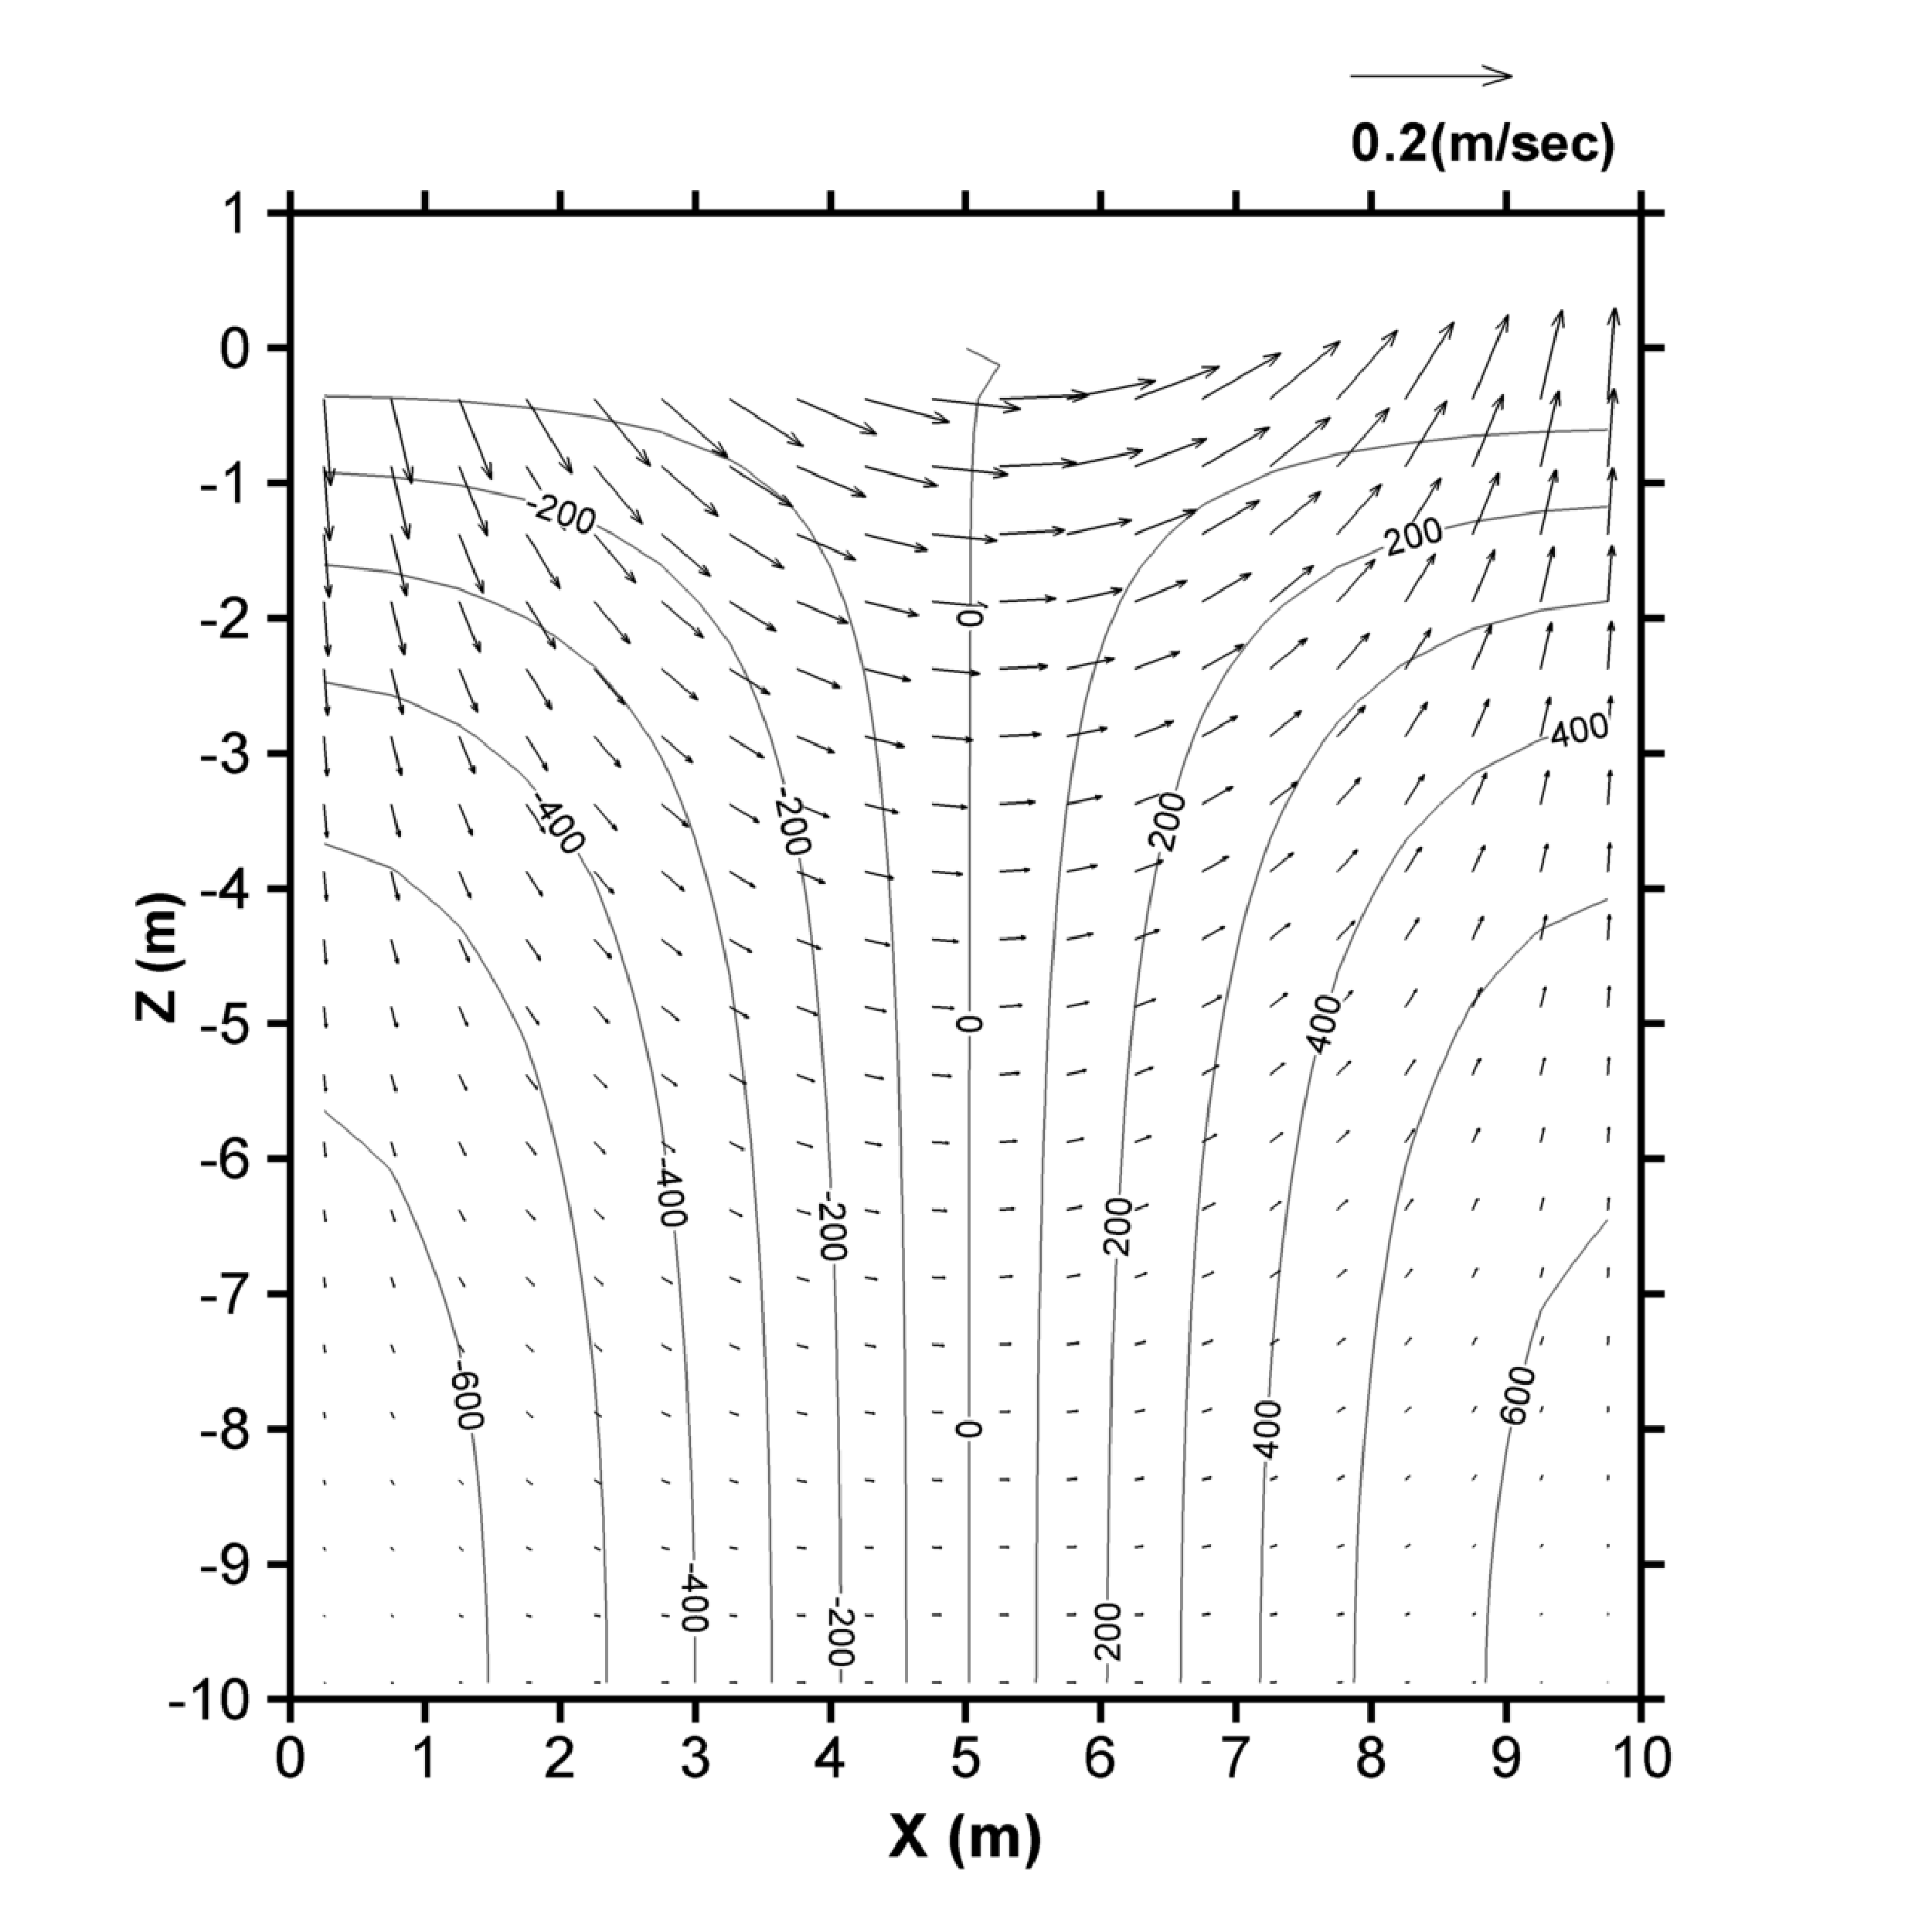
\includegraphics[width=3.2in]{../figures/StanWav/StanWav-Num-1-8.pdf}
}
\hspace{-0.5in}
\subfigure[Analytical] % caption for subfigure b
{
    \label{fig:sub:b}
    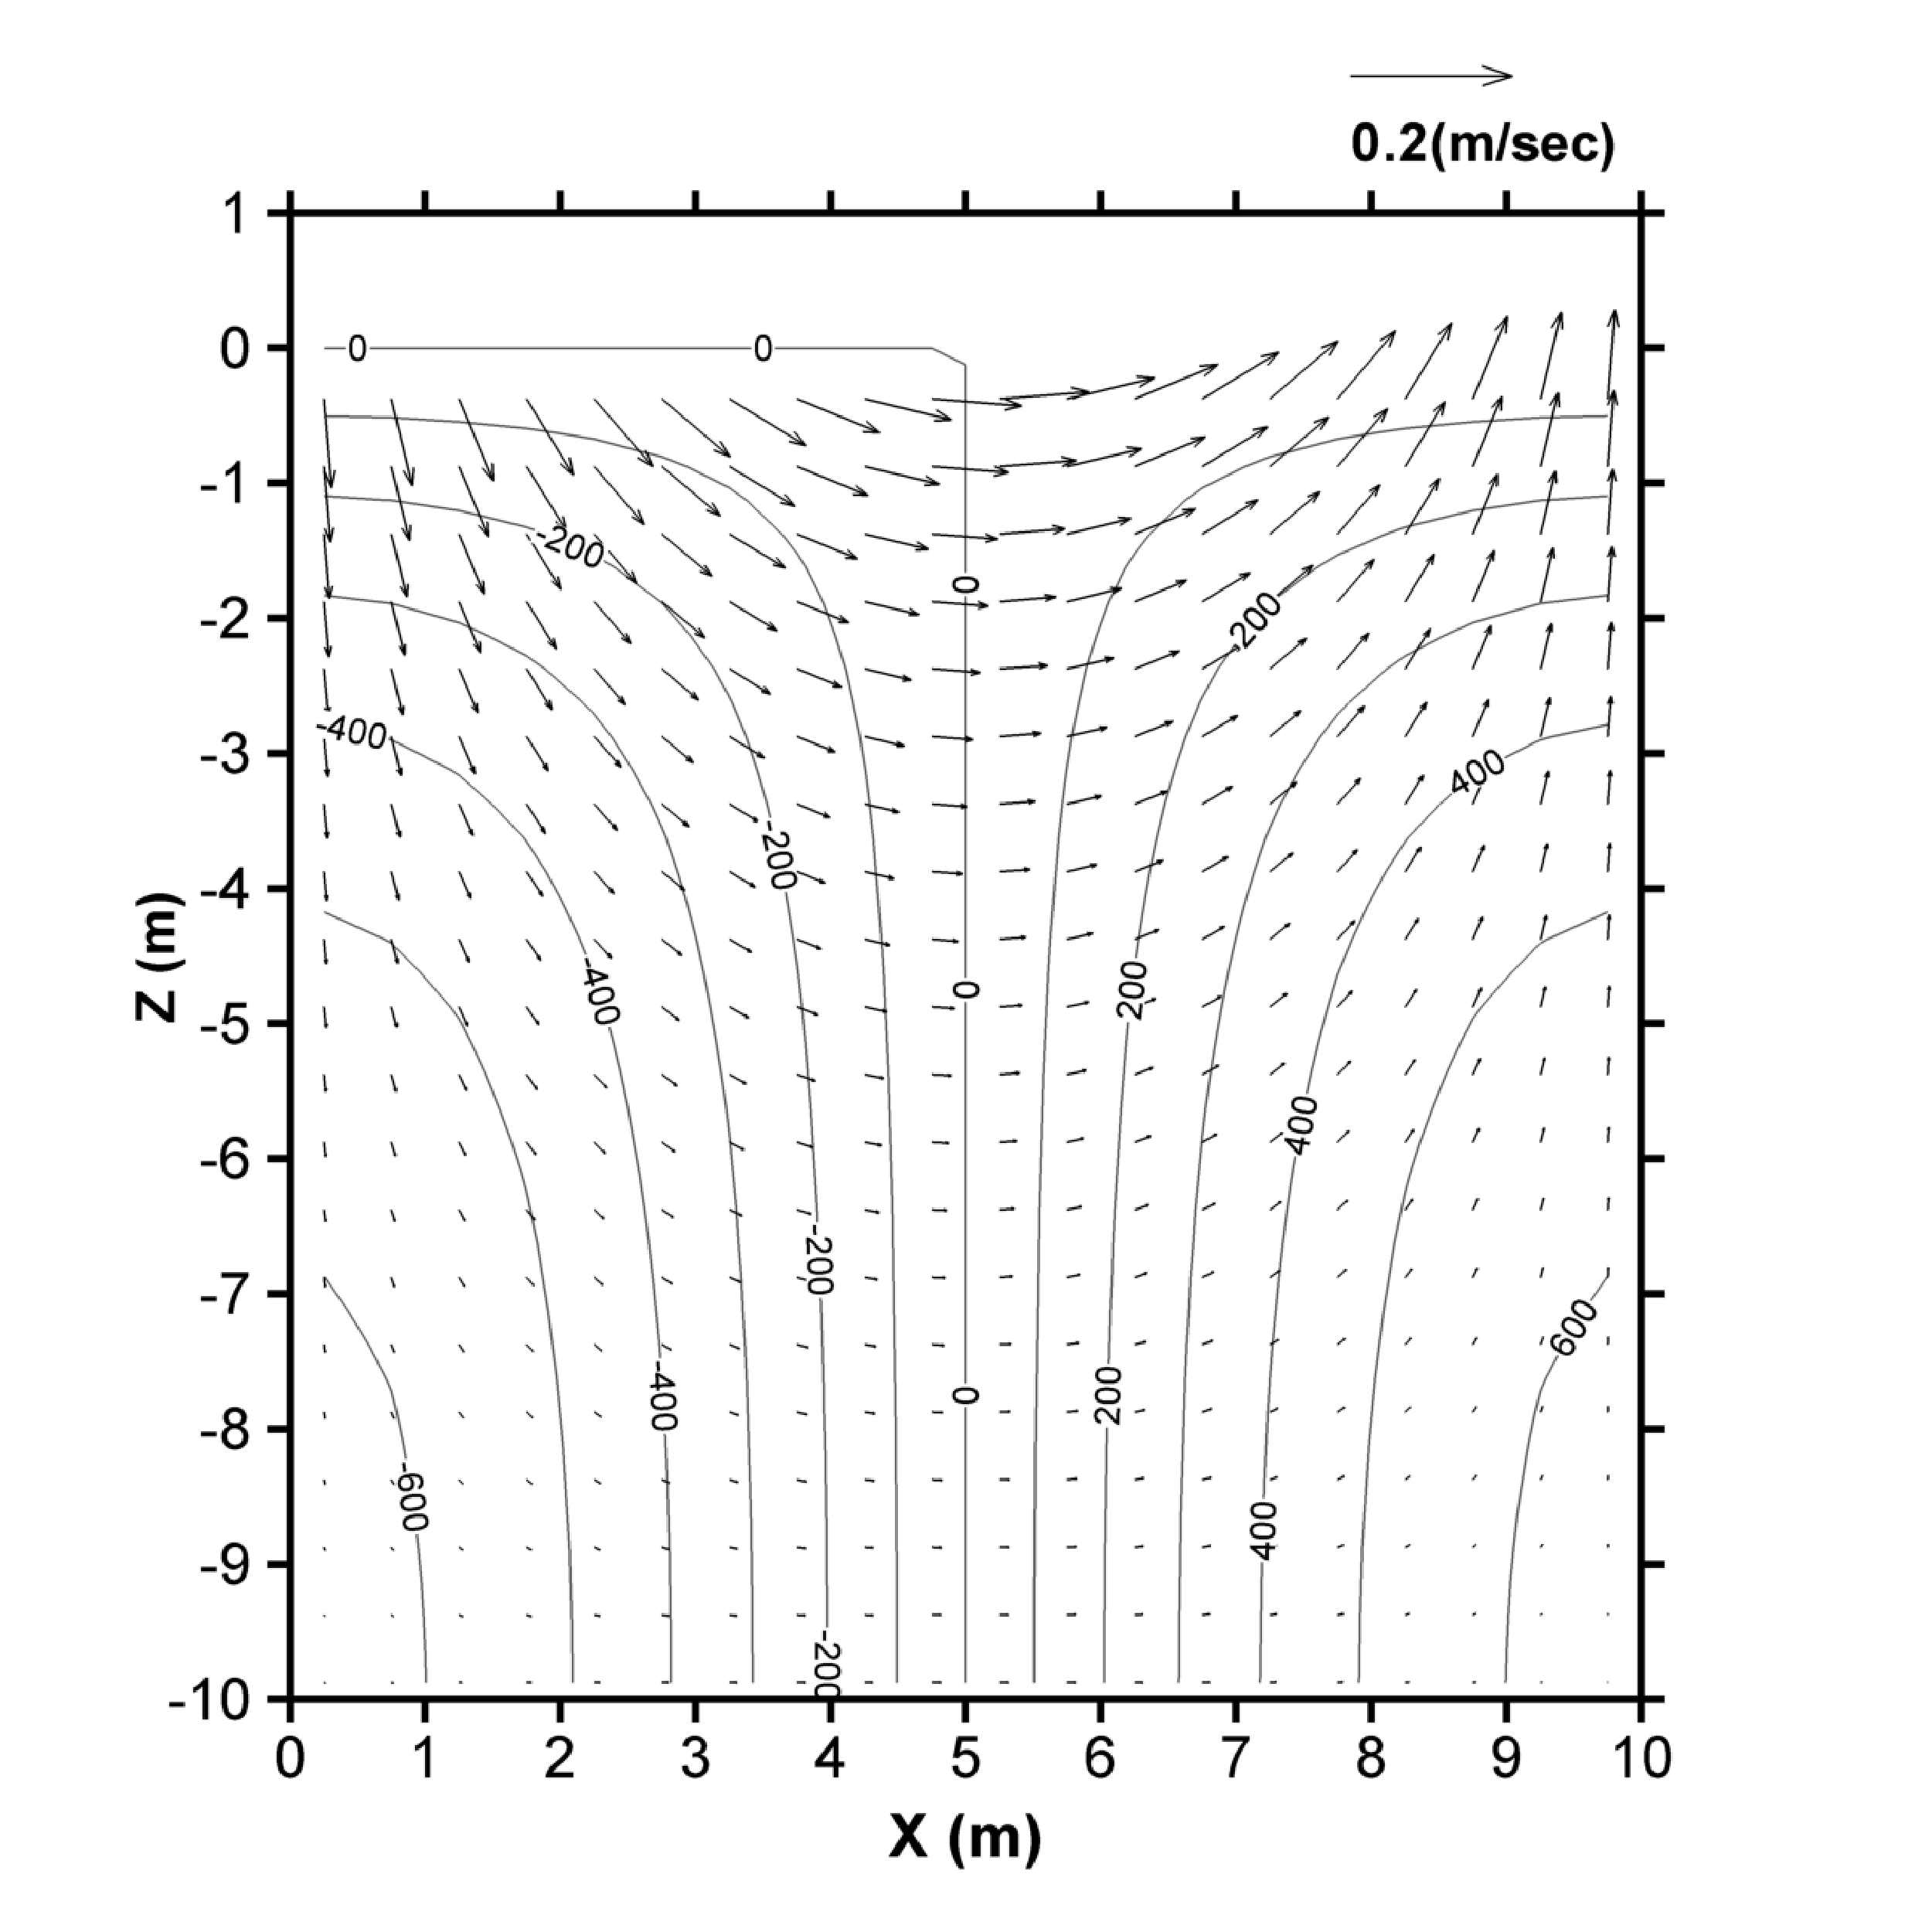
\includegraphics[width=3.2in]{../figures/StanWav/StanWav-Ana-1-8.pdf}
}
\caption{Standing wave test. Pressure and velocity plots at $t= 1/8 T$}
\label{fig:StanWav-1-8}
\vspace{0.3in}

\hspace{0.0in}
\subfigure[Numerical] % caption for subfigure a
{
    \label{fig:sub:a}
    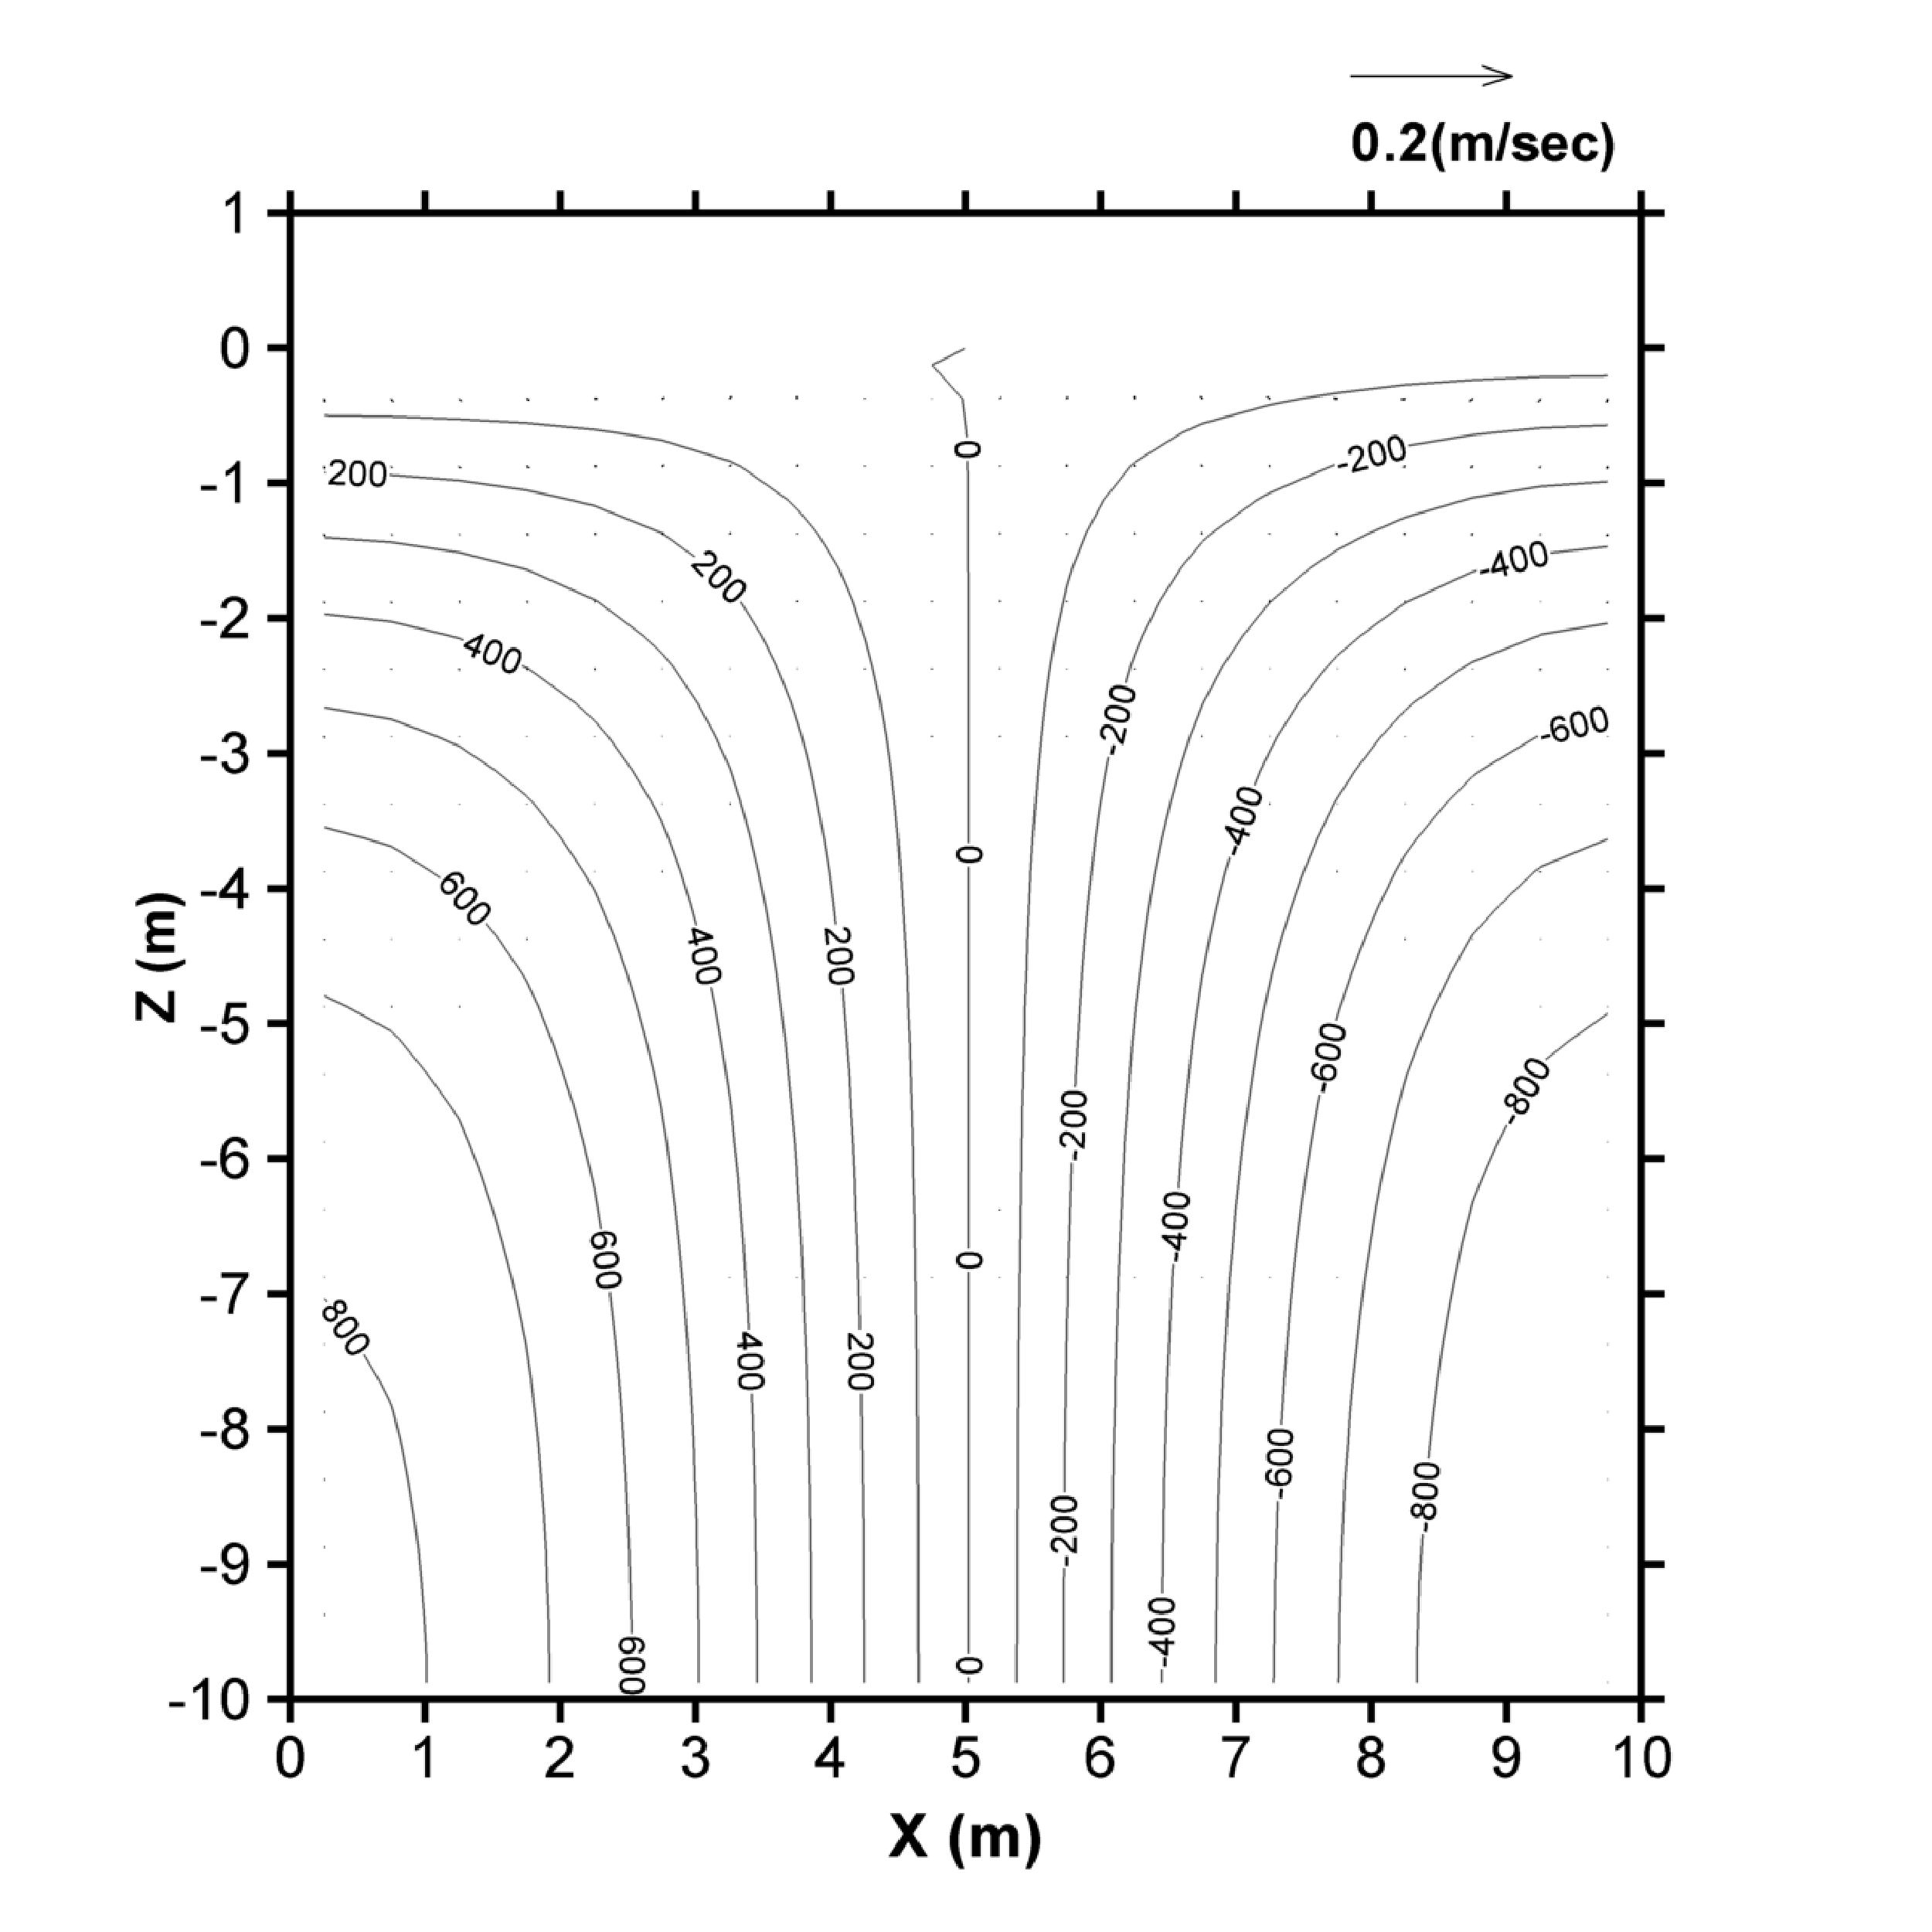
\includegraphics[width=3.2in]{../figures/StanWav/StanWav-Num-4-8.pdf}
}
\hspace{-0.5in}
\subfigure[Analytical] % caption for subfigure b
{
    \label{fig:sub:b}
    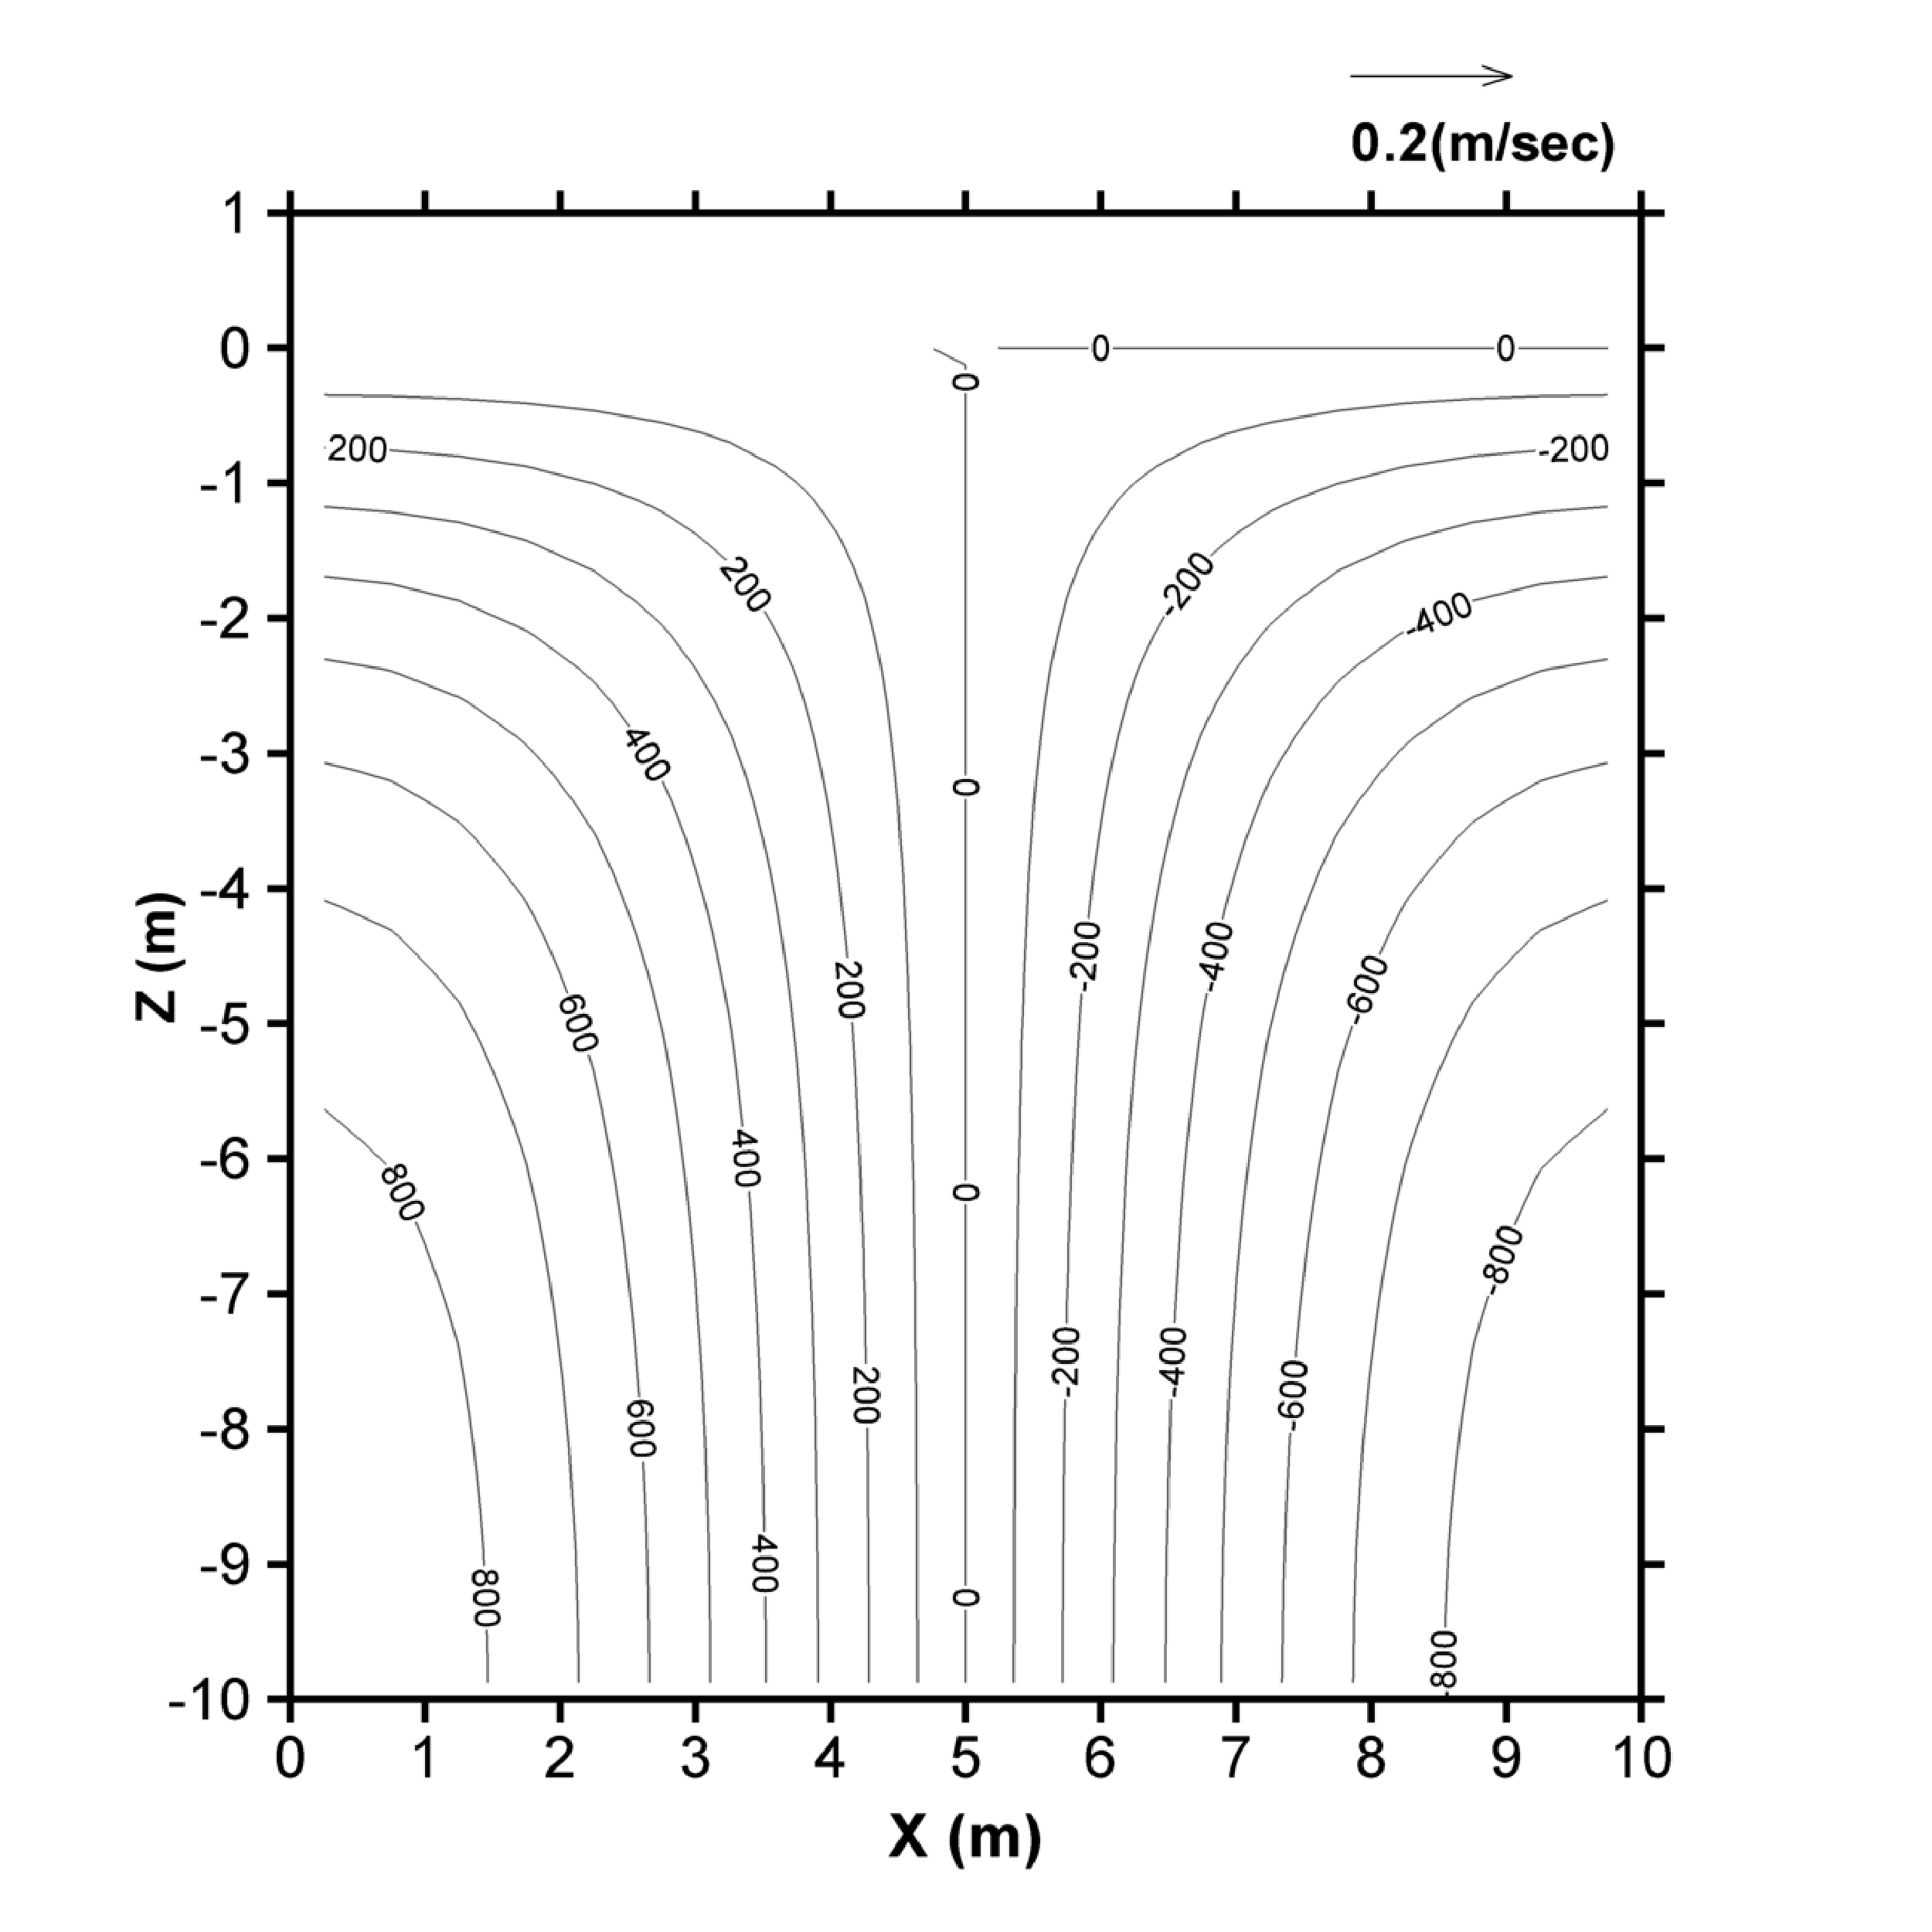
\includegraphics[width=3.2in]{../figures/StanWav/StanWav-Ana-4-8.pdf}
}
\caption{Standing wave test. Pressure and velocity plots at $t= 1/2 T$}
\label{fig:StanWav-4-8}
\end{figure}



\begin{figure}[htbp]
\vspace{-0.2in}
\hspace{0.0in}
\subfigure[Numerical] % caption for subfigure a
{
    \label{fig:sub:a}
    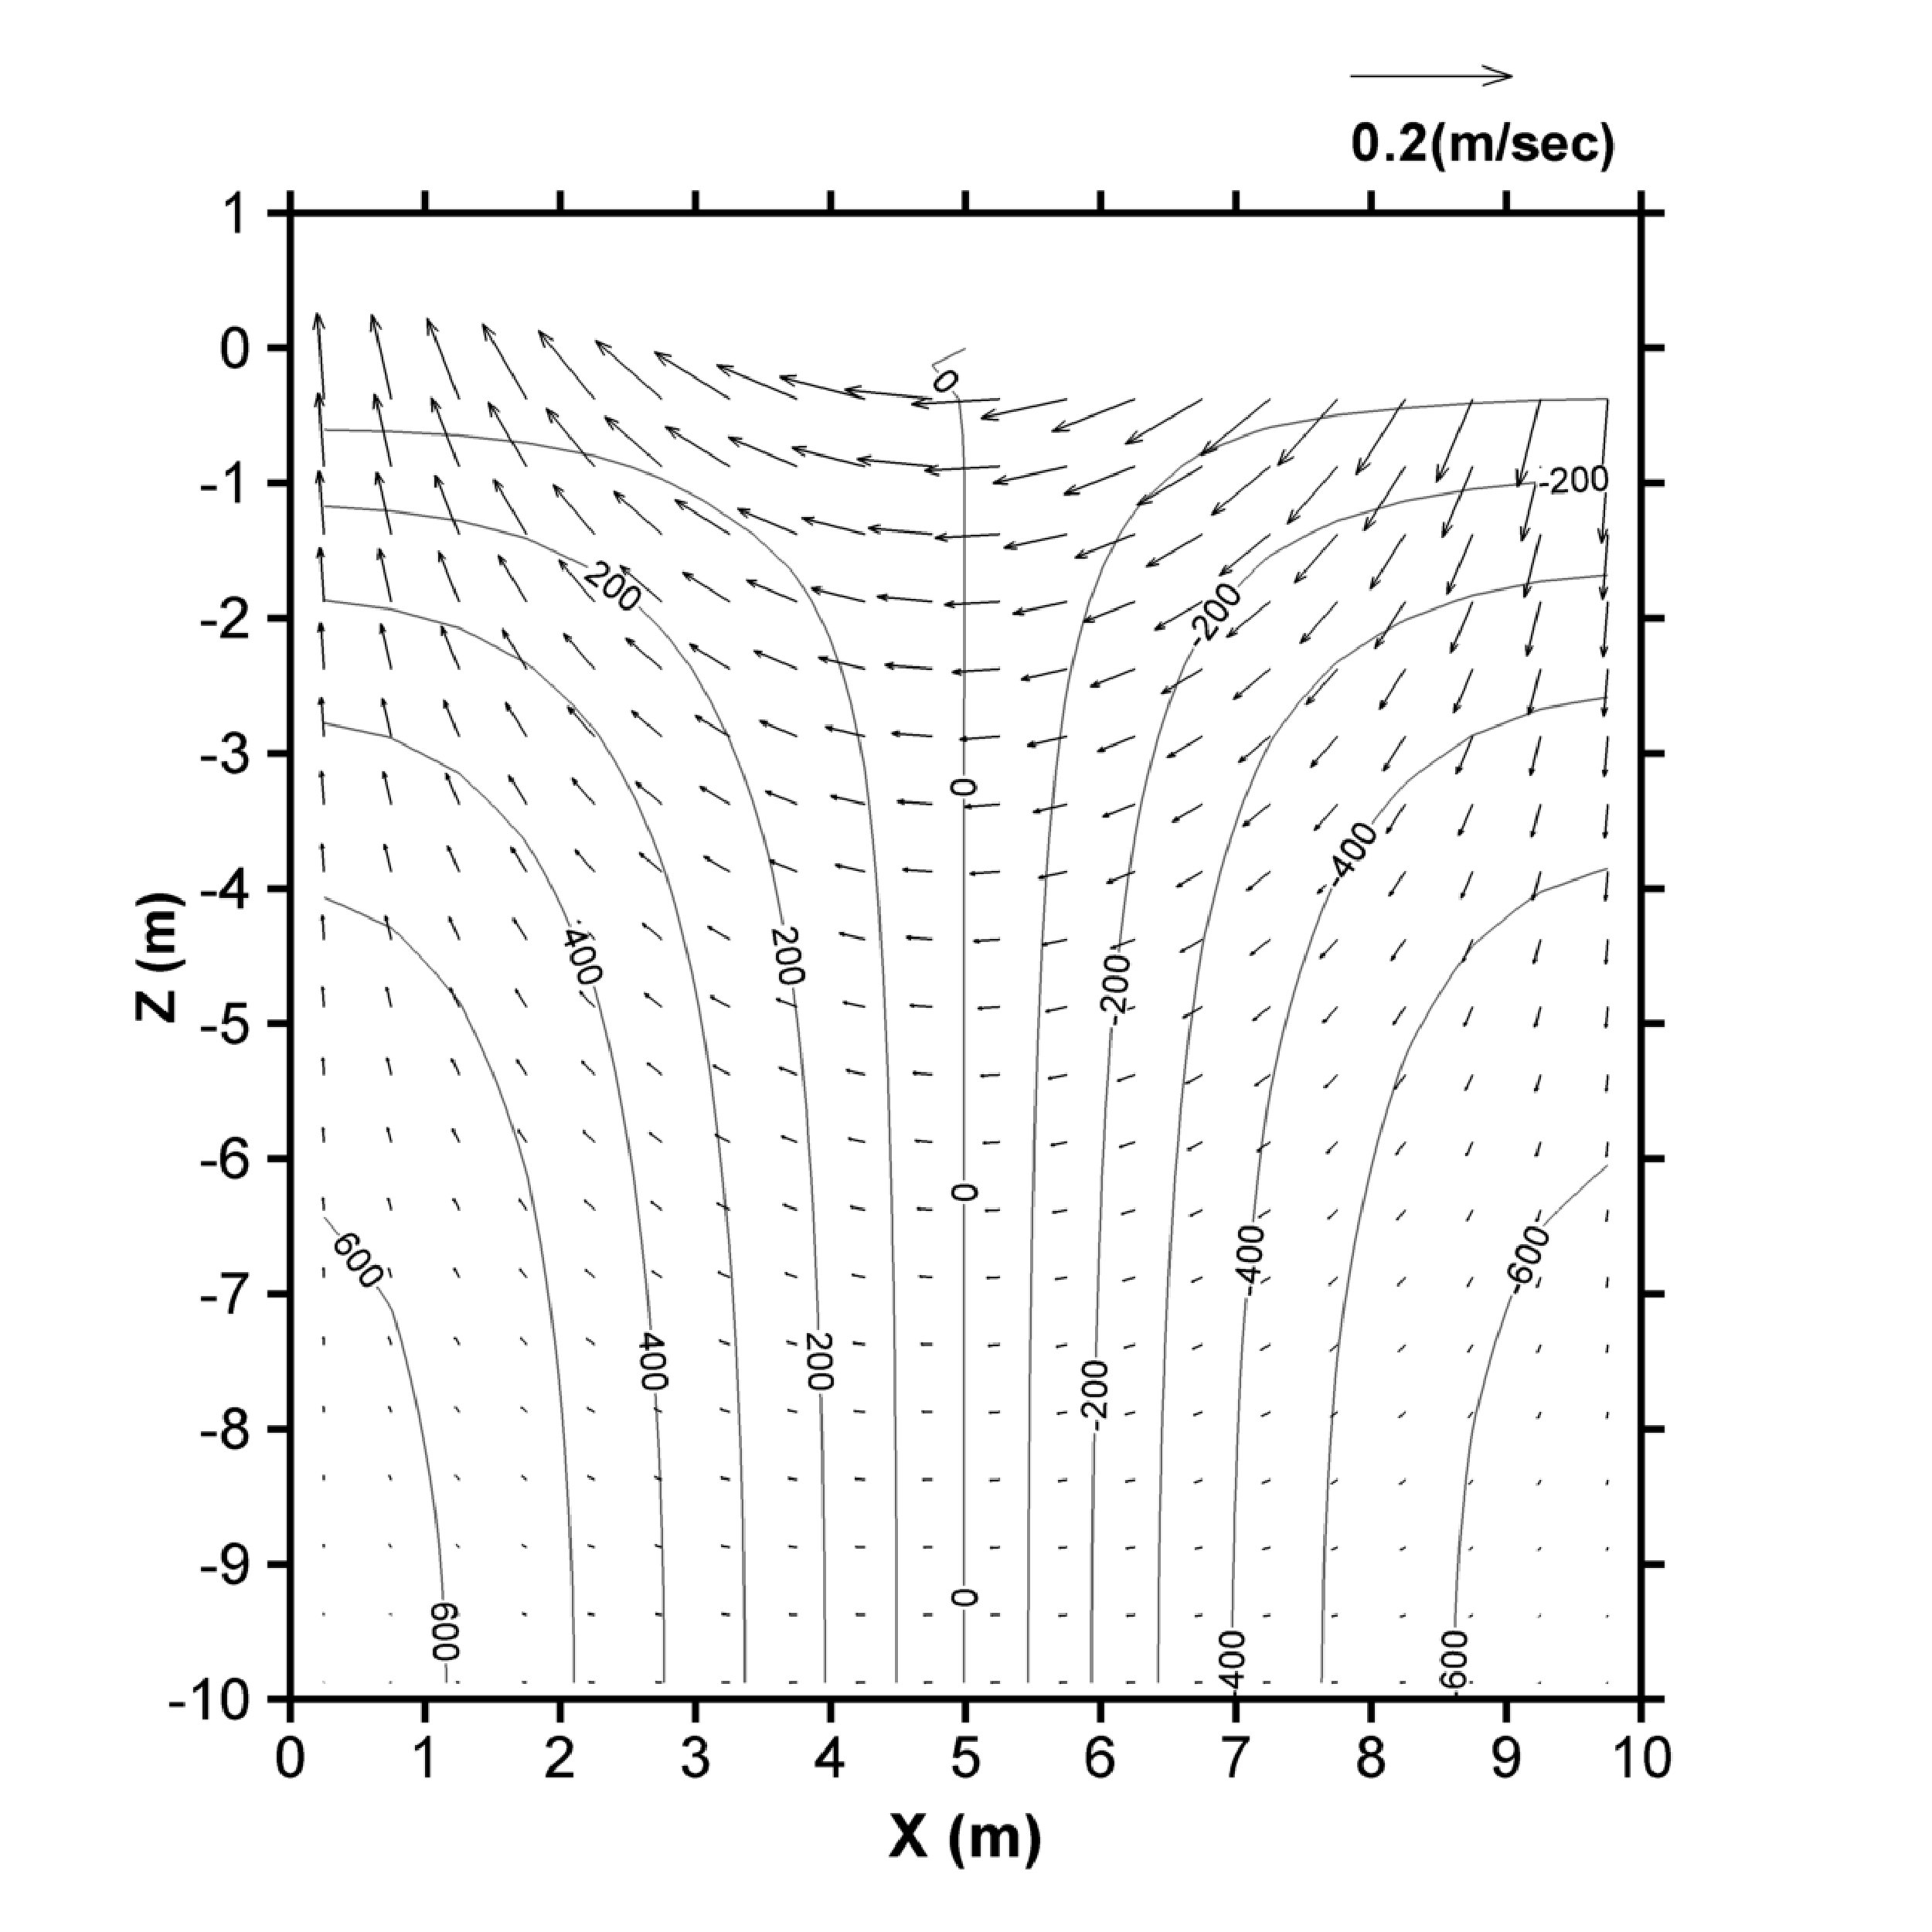
\includegraphics[width=3.2in]{../figures/StanWav/StanWav-Num-5-8.pdf}
}
\hspace{-0.5in}
\subfigure[Analytical] % caption for subfigure b
{
    \label{fig:sub:b}
    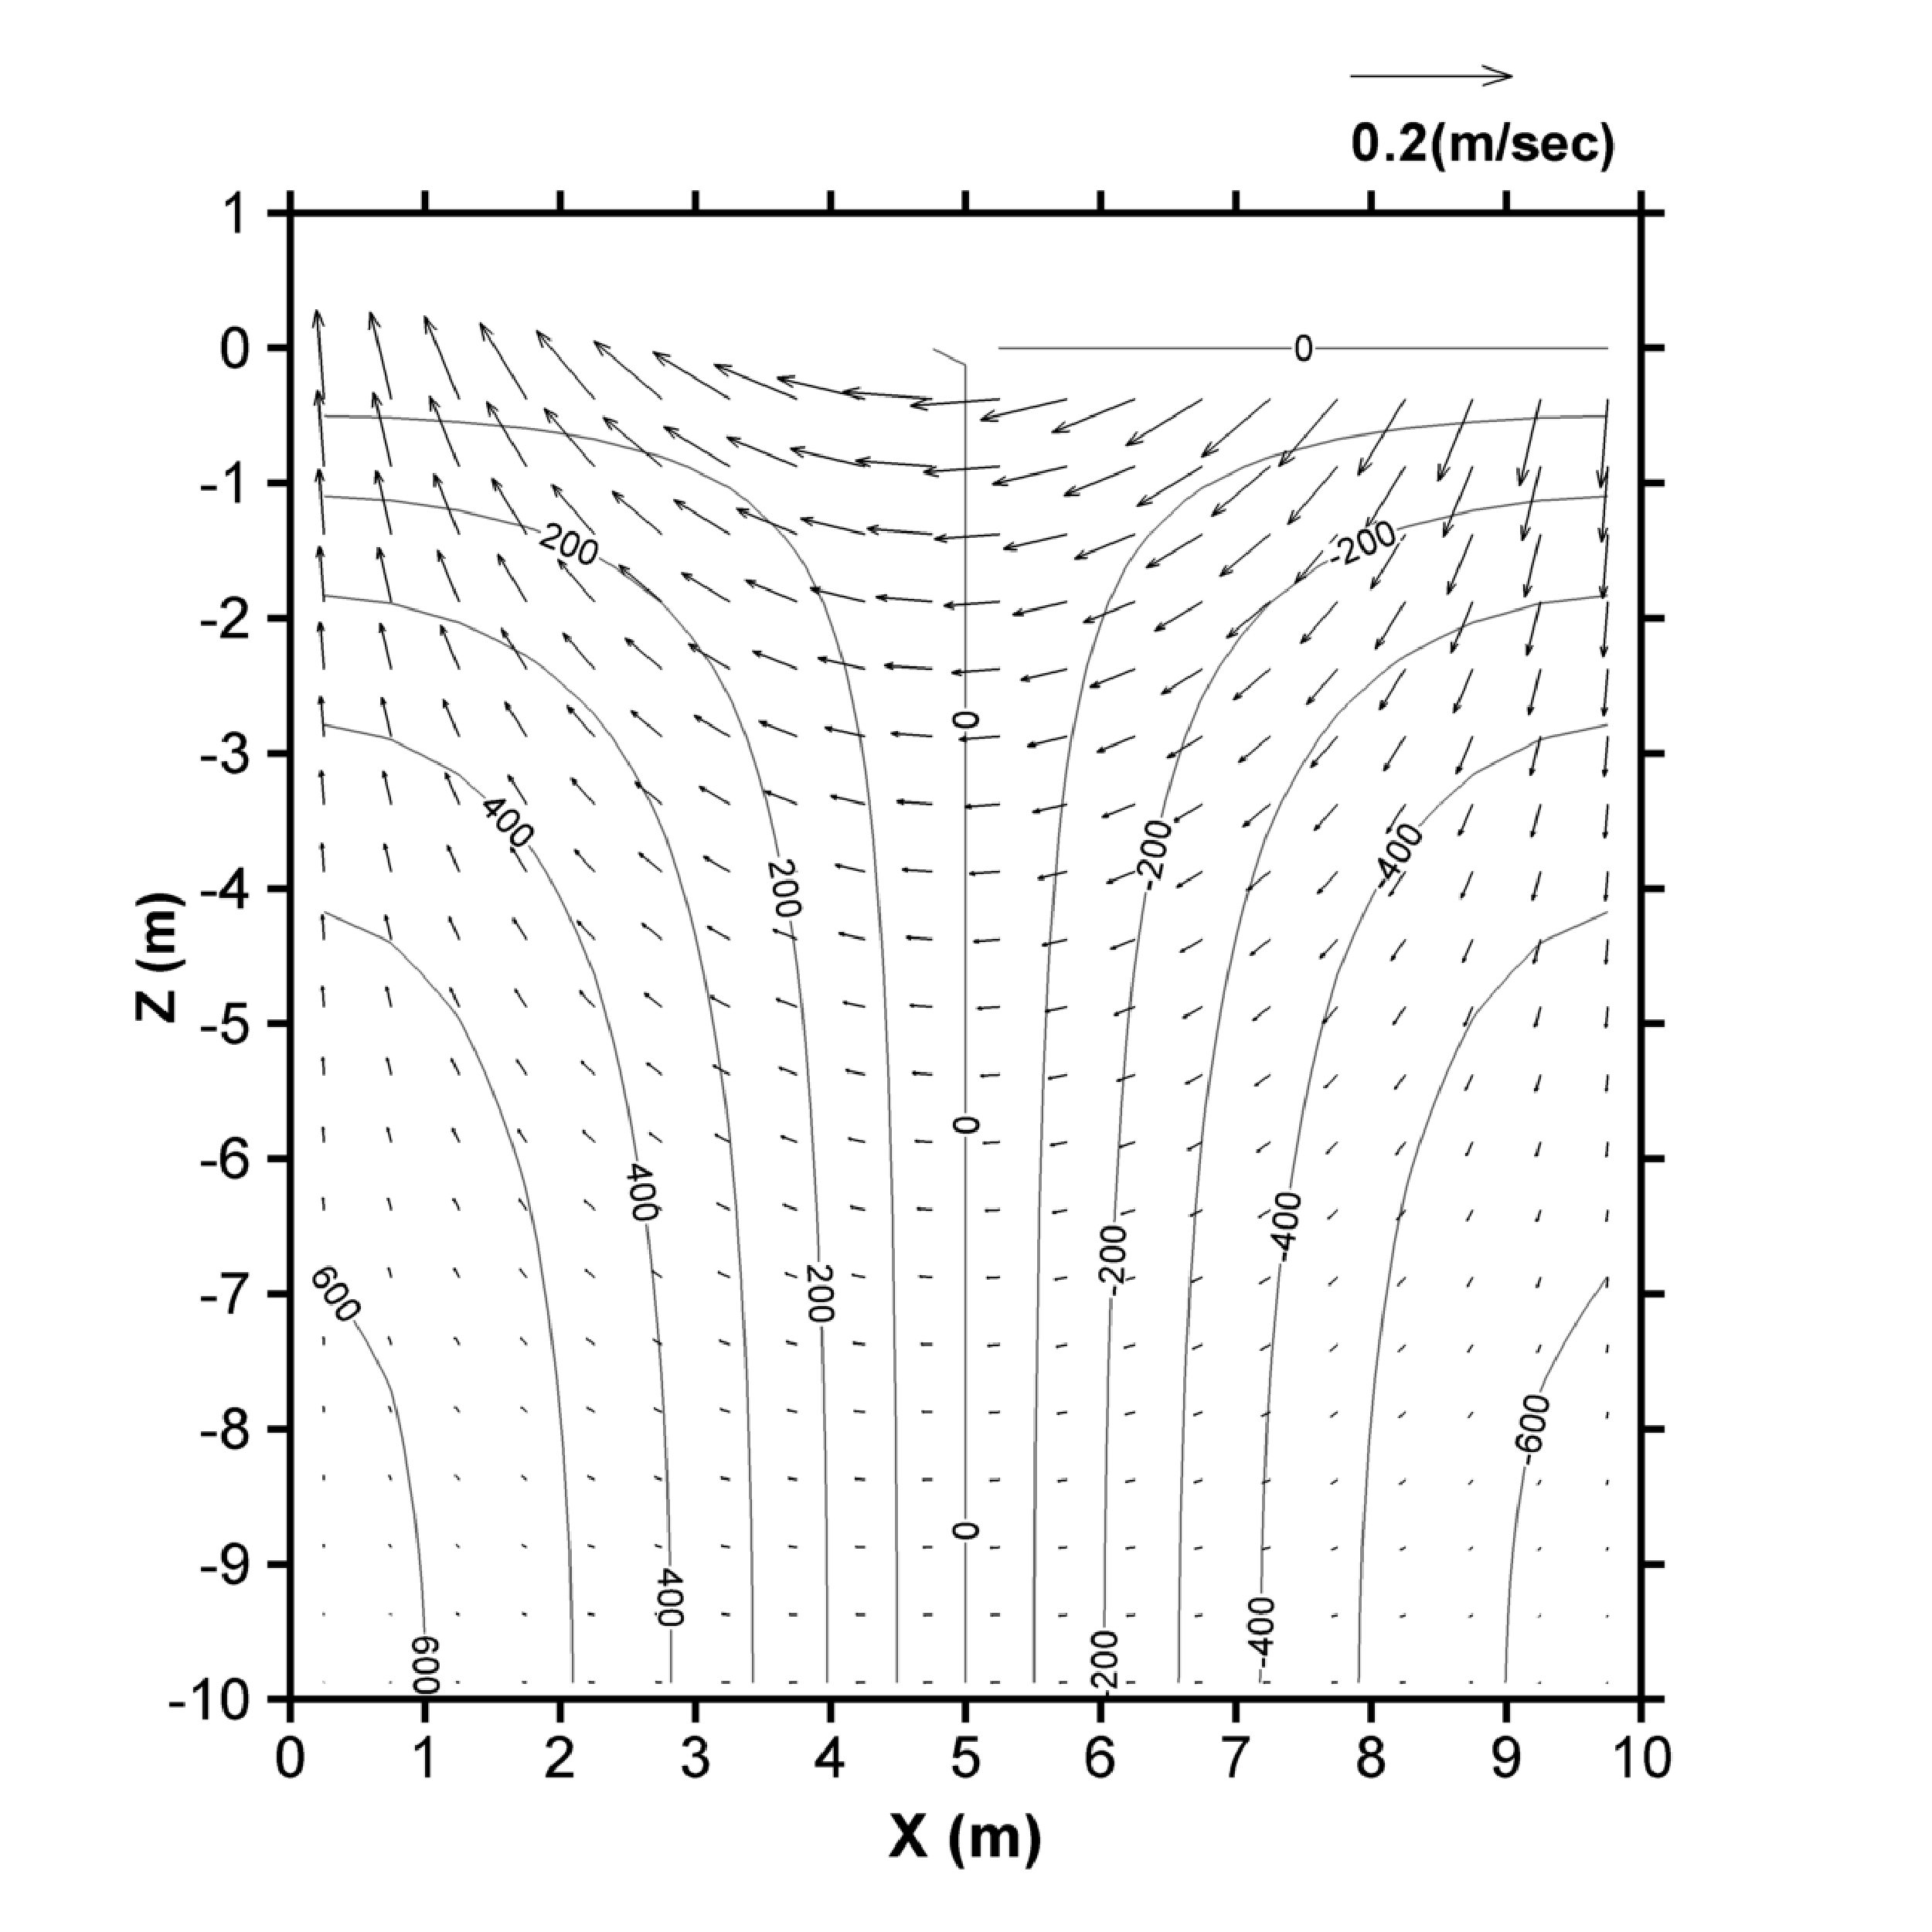
\includegraphics[width=3.2in]{../figures/StanWav/StanWav-Ana-5-8.pdf}
}
\caption{Standing wave test. Pressure and velocity plots at $t= 5/8 T$}
\label{fig:StanWav-5-8} % caption for the whole figure

\vspace{0.25in}
\hspace{0.0in}
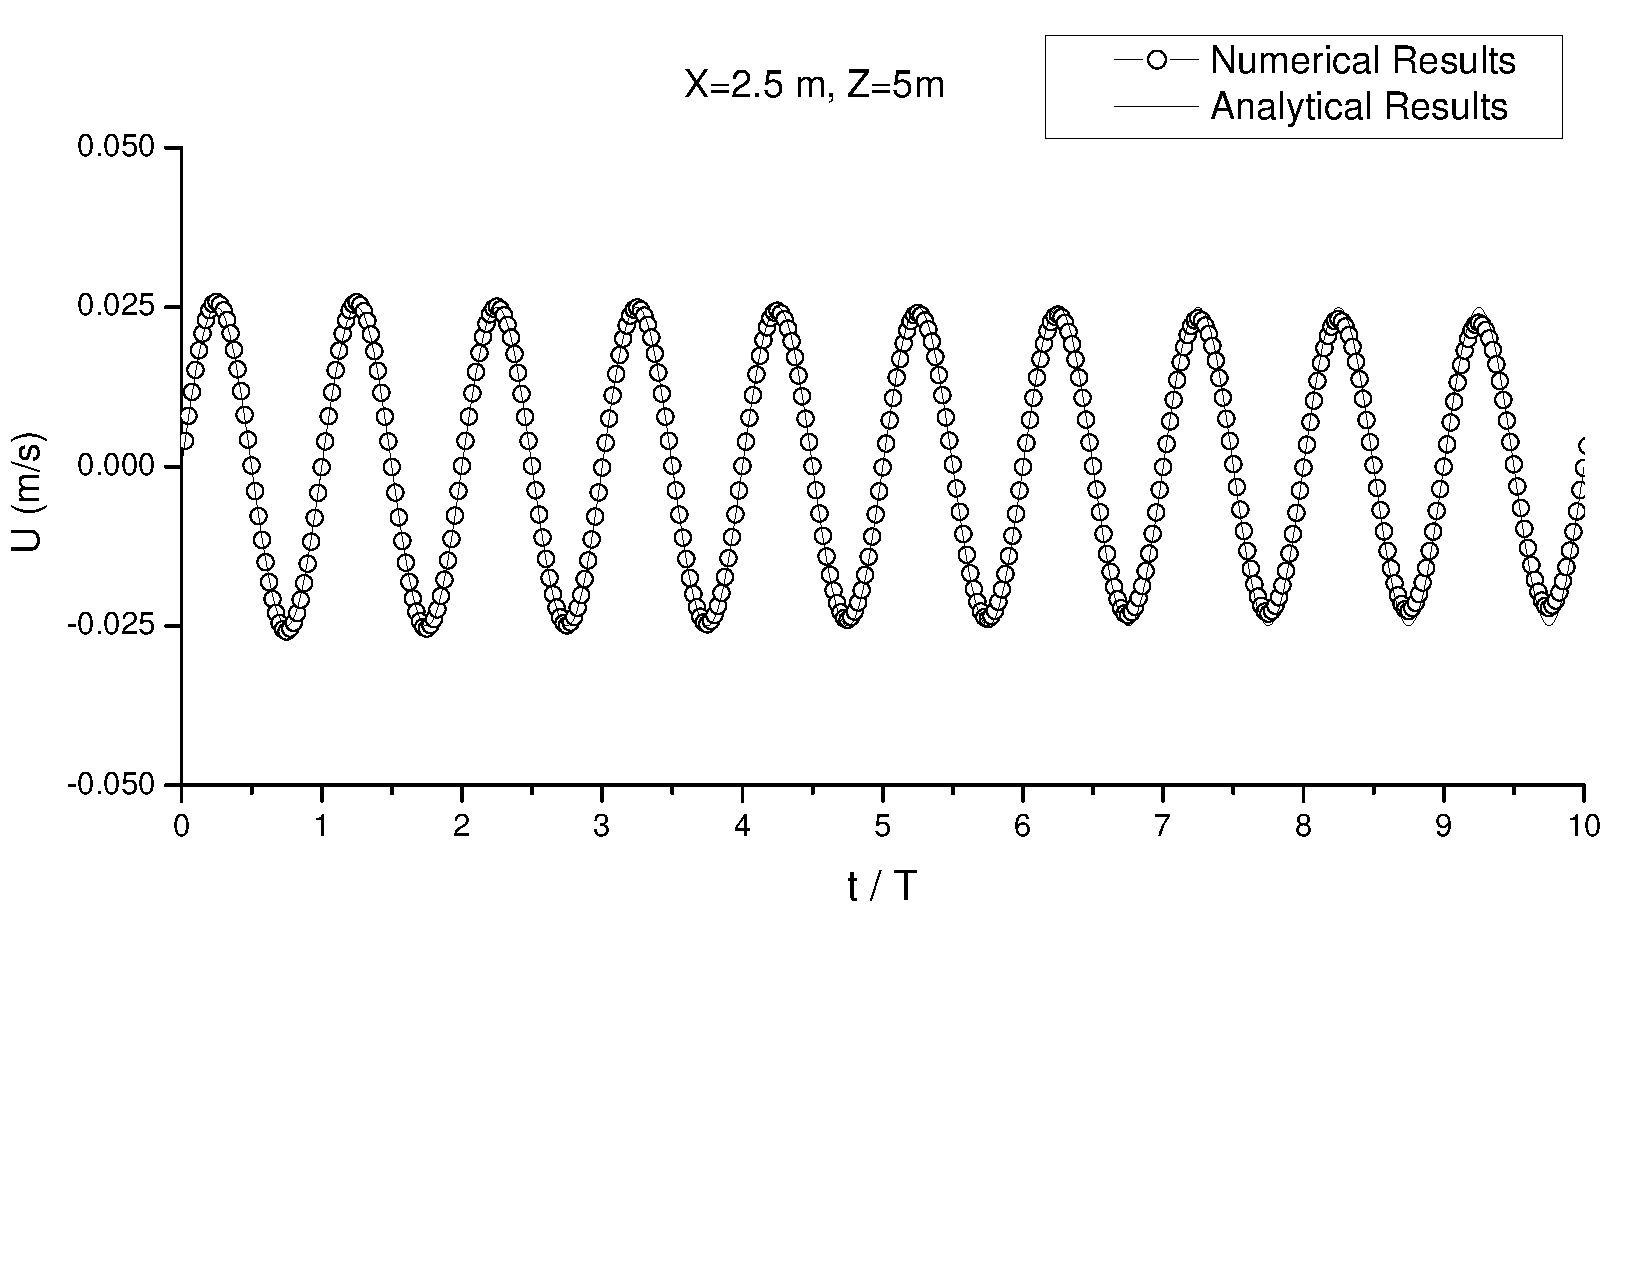
\includegraphics[scale=0.50]{../figures/StanWav/StanWav-U-vs-Time-X=25-Z=5.pdf}
\label{fig:StanWav-U-vs-Time-X-25-Z-5}
\caption{Standing wave test. Velocity $u$ versus time}
\end{figure}

\cp

\begin{figure}[htbp]
\begin{center}
\vspace{0.3in}
\hspace{0.0in}
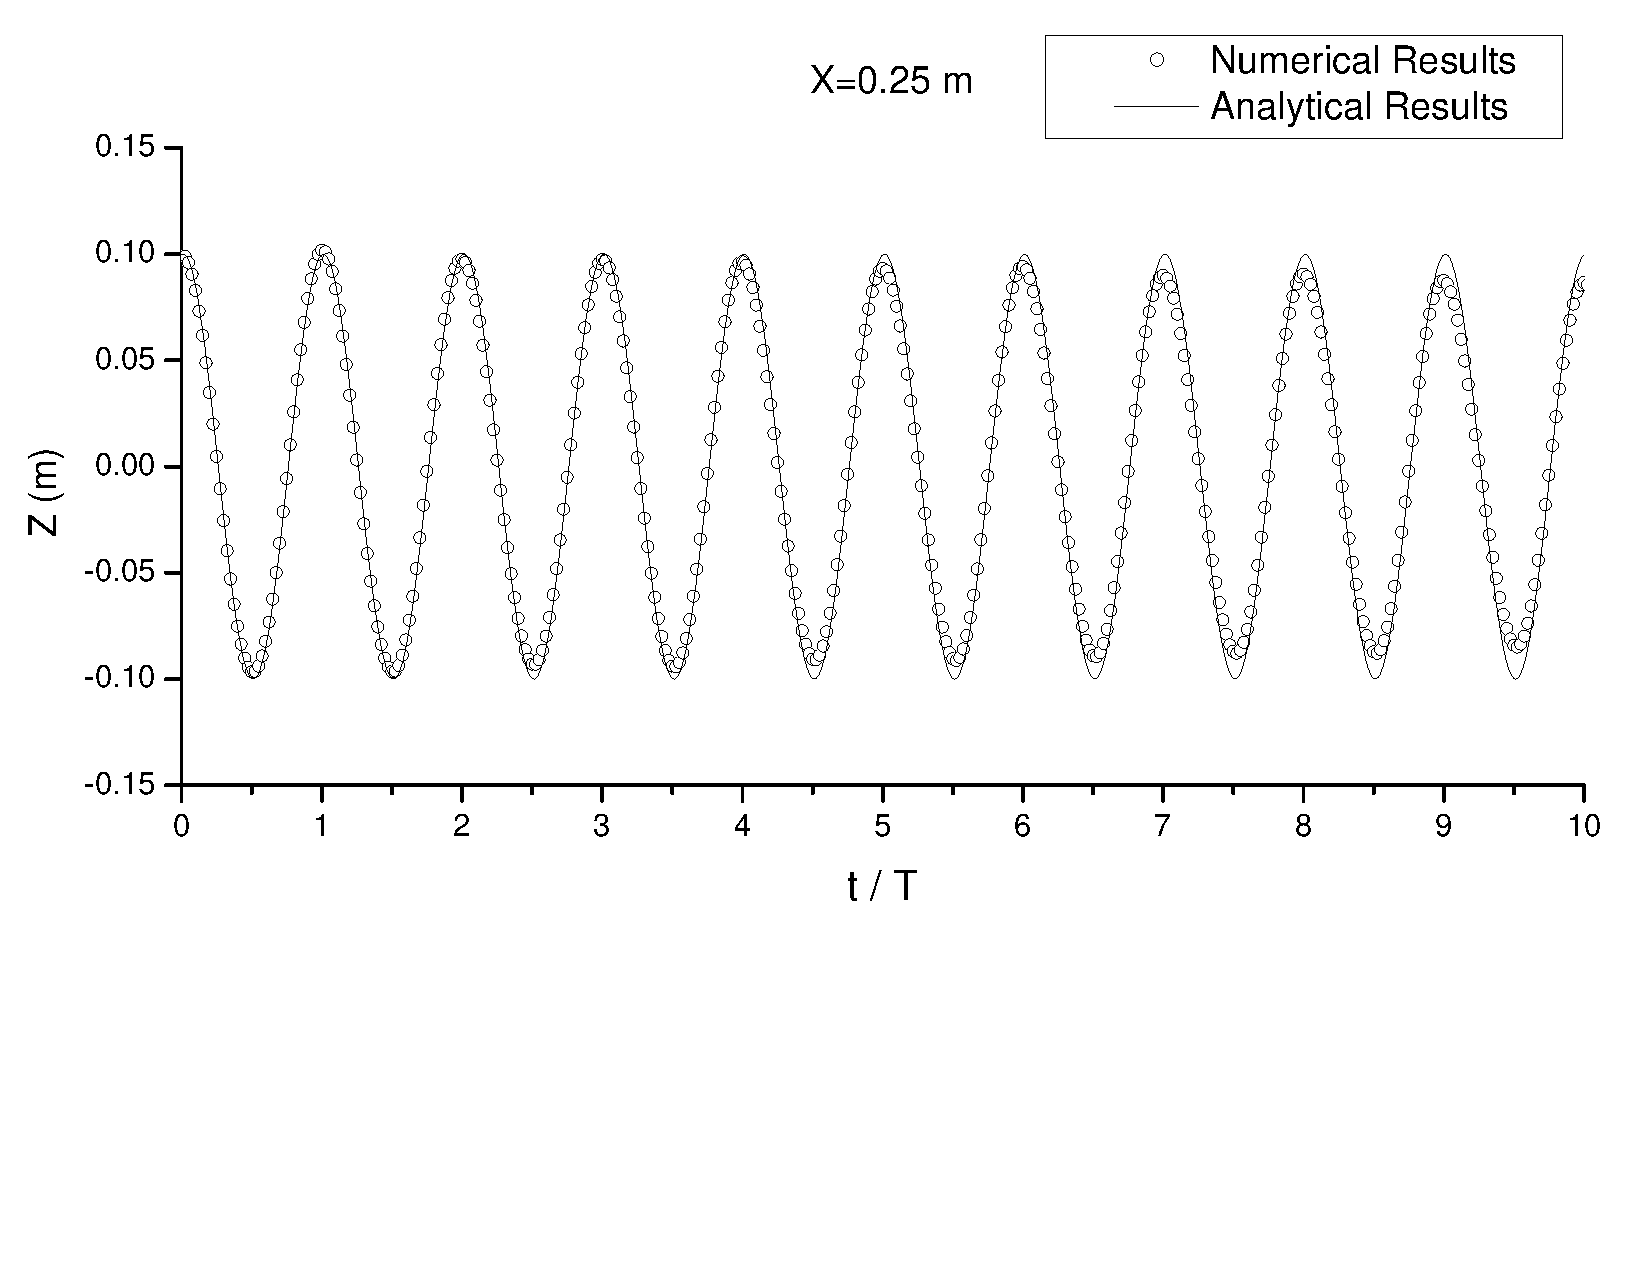
\includegraphics[scale=0.50]{../figures/StanWav/StanWav-Height-vs-Time-x=025.pdf}
\vspace{0.5in}
\hspace{0.0in}
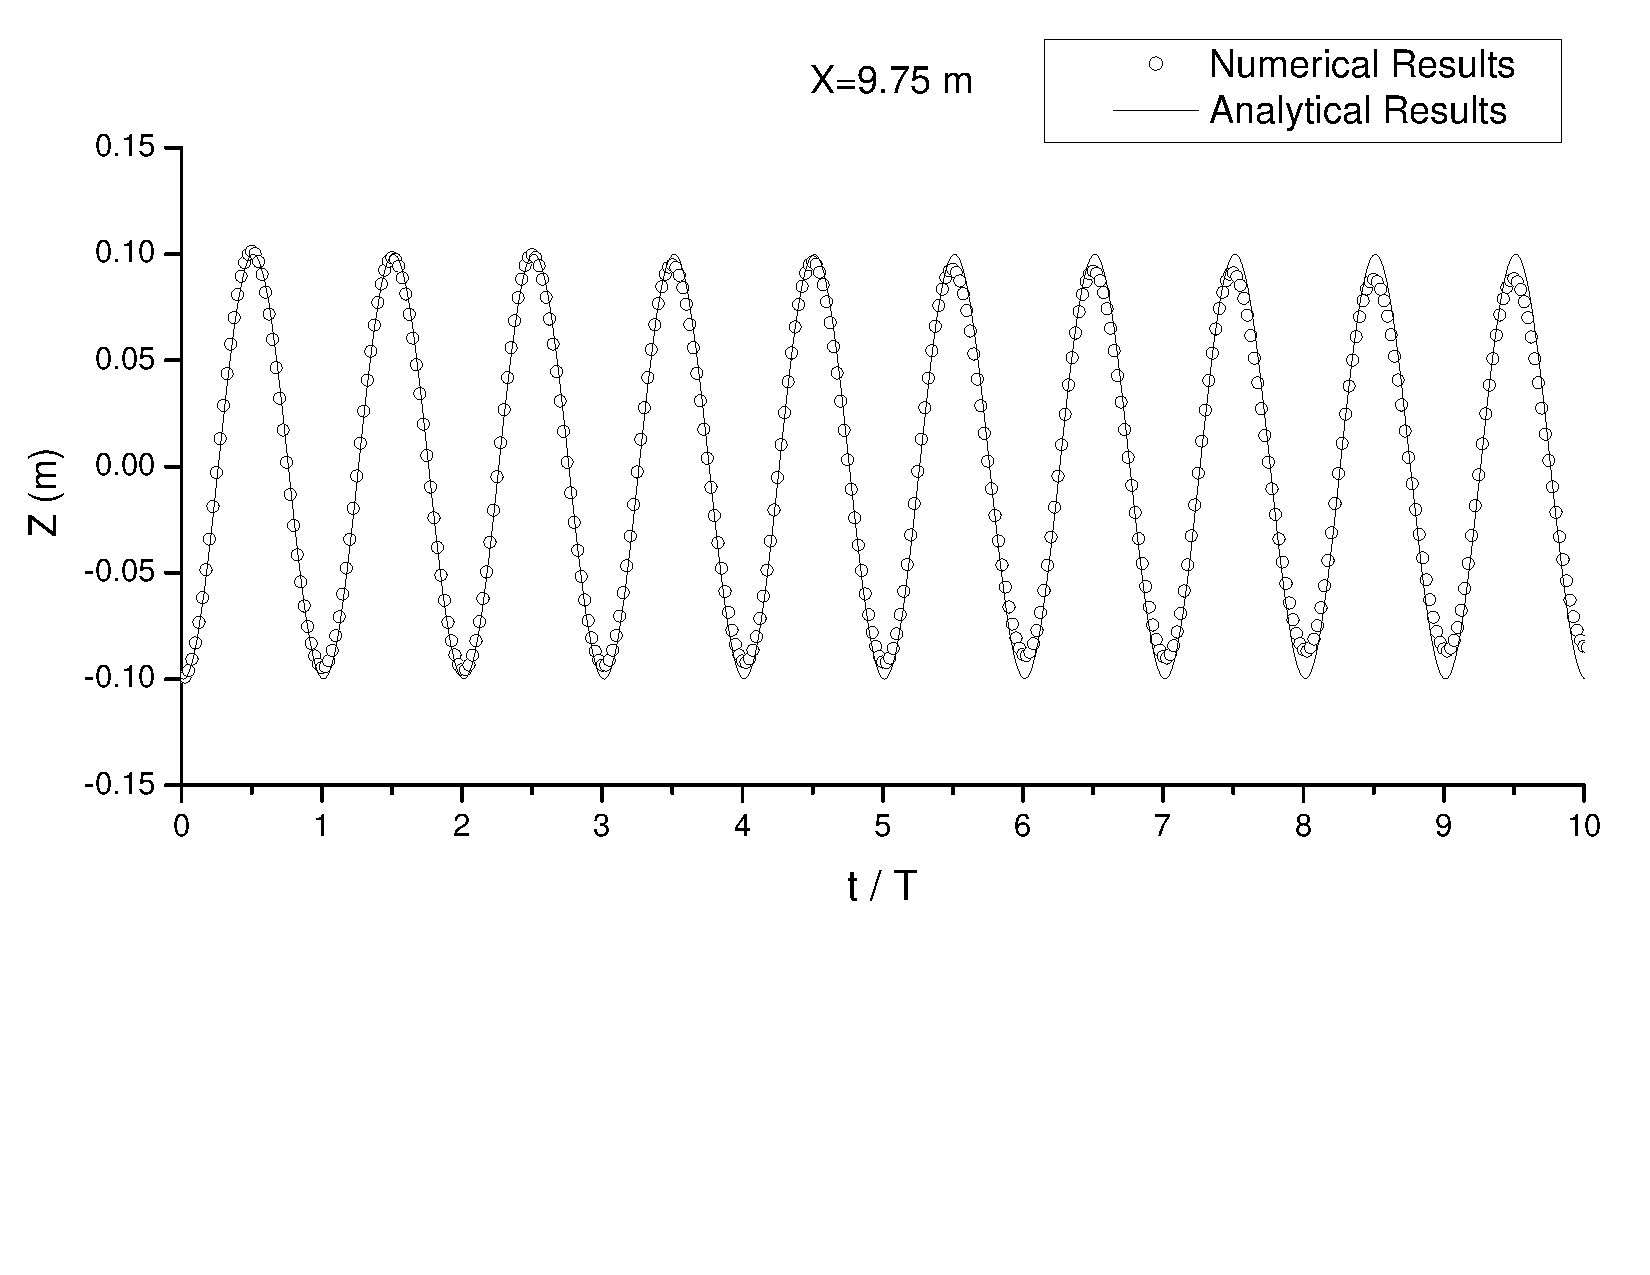
\includegraphics[scale=0.50]{../figures/StanWav/StanWav-Height-vs-Time-x=975.pdf}
\caption{Standing wave test. Surface level versus time}
\label{fig:StanWav-Height-vs-Time}
\end{center}
\end{figure}

\cp

\begin{table}[h]
\vspace{0.8in}
\caption{Grid convergence test. Velocities $u$ of different grid resolutions}
\begin{center}
\begin{tabular}{cccccc} \hline
x(m) & z(m) & 243*243 & 81*81 & 27*27 & 9*9  \\ \hline
2.7 & -6.75 &  2.631E-04  & 2.647E-04  & 2.833E-04  & 3.218E-04 \\
2.7 & -4.05 &  5.801E-04  & 5.881E-04  & 6.175E-04  & 6.939E-04 \\
2.7 & -1.35 &  1.595E-03  & 1.616E-03  & 1.681E-03  & 1.879E-03 \\
5.4 & -6.75 &  2.633E-04  & 2.638E-04  & 2.794E-04  & 3.231E-04 \\
5.4 & -4.05 &  5.803E-04  & 5.873E-04  & 6.143E-04  & 6.950E-04 \\
5.4 & -1.35 &  1.595E-03  & 1.616E-03  & 1.680E-03  & 1.879E-03 \\
\hline
\end{tabular}

\vspace{0.8in}
\caption{Grid convergence test. Velocities $w$ of different grid resolutions}
\begin{tabular}{cccccc} \hline
x(m) & z(m) & 243*243 & 81*81 & 27*27 & 9*9 \\ \hline
1.35  &  -5.4  &  -2.894E-04  & -2.956E-04  & -3.065E-04 & 3.218E-04 \\
4.05  &  -5.4  &  -6.471E-08  & -1.254E-07  & -6.886E-07 & 6.939E-04 \\
6.75  &  -5.4  &  2.892E-04   & 2.954E-04   & 3.056E-04  & 1.879E-03 \\
1.35  &  -2.7  &  -9.262E-04  & -9.383E-04  & -9.720E-04 & 3.231E-04 \\
4.05  &  -2.7  &  -1.769E-07  & 4.434E-08   & -1.889E-07 & 6.950E-04 \\
6.75  &  -2.7  &  9.258E-04   & 9.389E-04   & 9.735E-04  & 1.879E-03 \\
\hline
\end{tabular}
\end{center}
\end{table}

\cp

\begin{table}
\begin{center}
\vspace{0.5in}
\caption{Grid convergence test. Error of velocities for different grid resolutions}
\small
\begin{tabular}{ccccccc} \hline
NX*NZ & $\Delta x(m)$  & $log \ error_2(u)$ &  $log \ error_1(u)$ & $log \ error_2(w)$ & $log \ error_1(w)$ \\ \hline
9*9  & 0.9 & -3.8162  & -3.7441 & -4.1301 & -3.9981 \\
27*27& 0.3 & -4.3314  & -4.2613 & -4.6723 & -4.5422 \\
81*81& 0.1 & -5.0039  & -4.8864 & -5.1988 & -5.0900 \\
\hline
\end{tabular}
\end{center}
\end{table}

\begin{figure}[h]
\vspace{0.8in}
\begin{center}
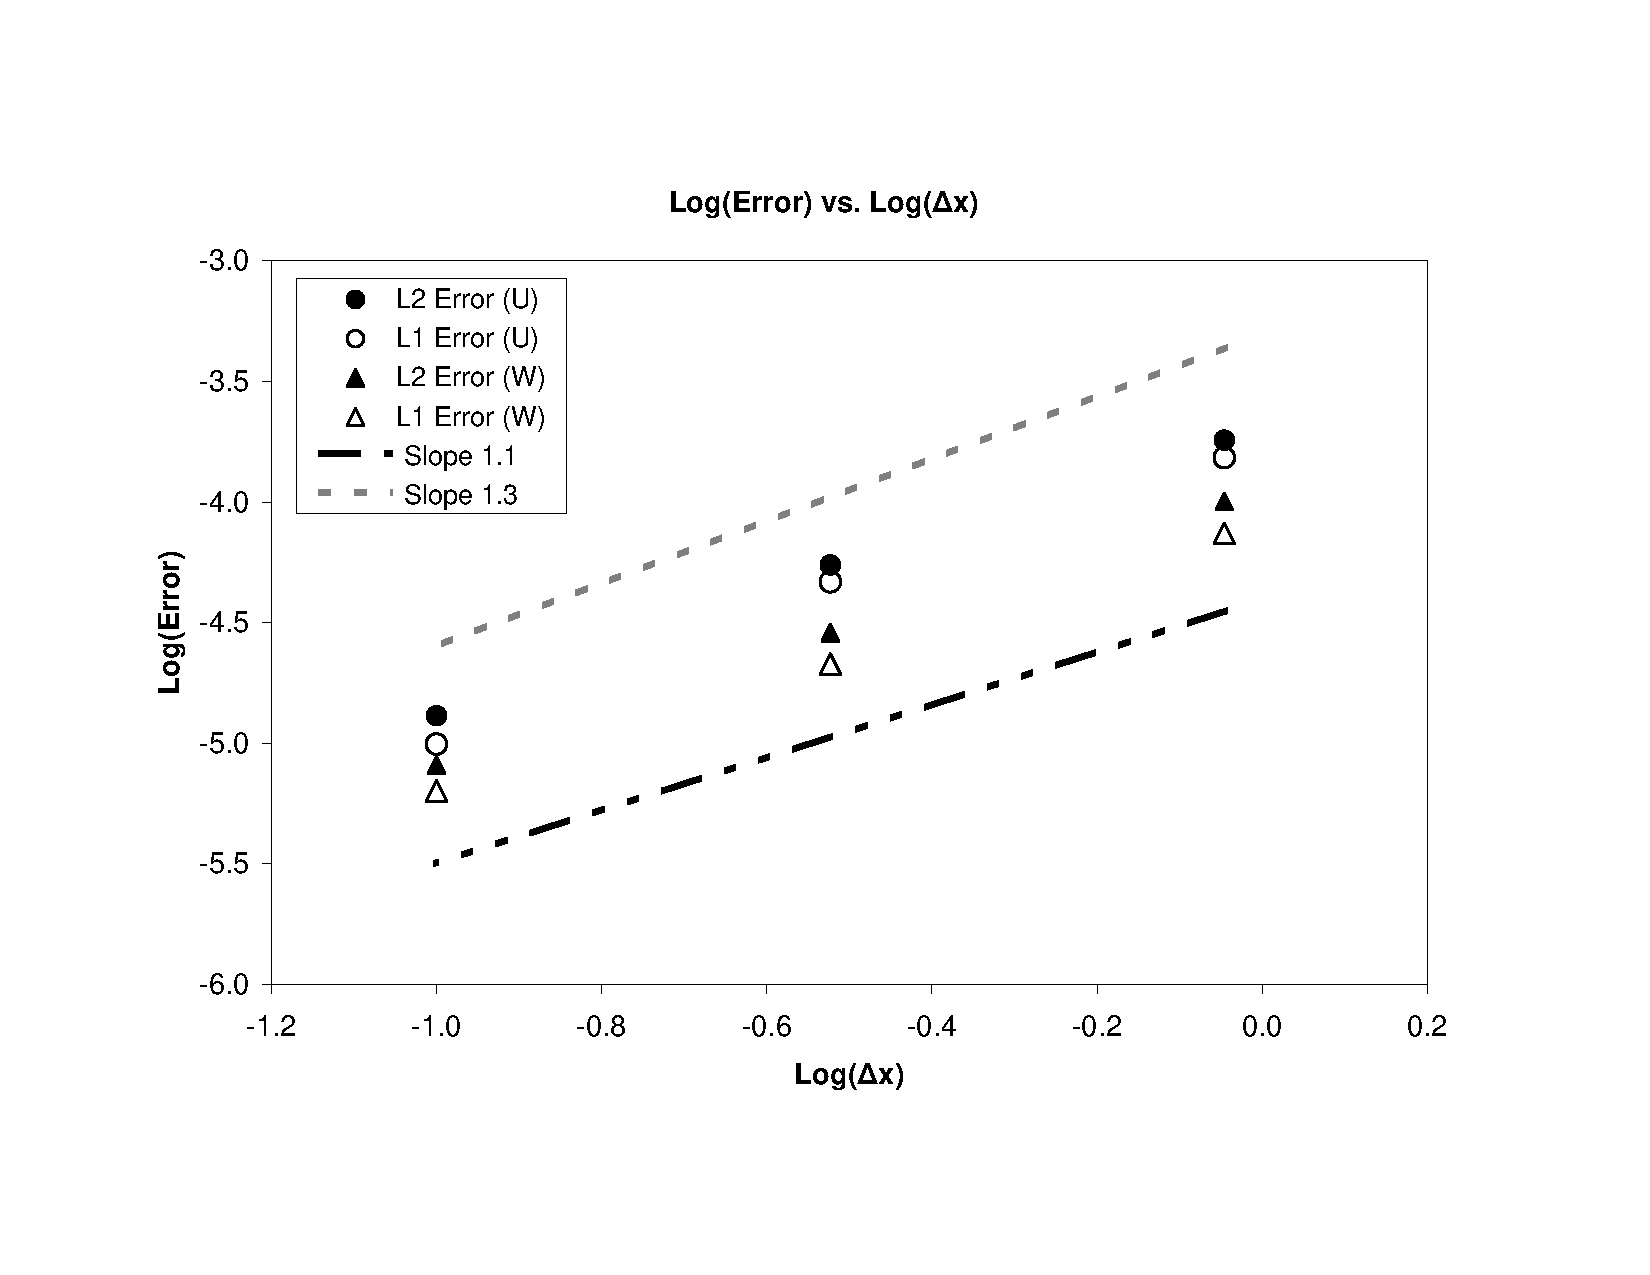
\includegraphics[width=5.4in]{../figures/GridConvTest/GridConvTest_dt0p01.pdf}
\label{fig:GridConvTest_dt0p01}
\vspace{-0.2in}
\caption{Grid Convergence Test.}
\end{center}
\end{figure}

\cp







\begin{comment}
\begin{table}[h]
\vspace{-0.2in}
\caption{Grid convergence test. Averaged velocities $u$ for different grid resolutions}
\small
\begin{center}
\begin{tabular}{cccccc} \hline
x(m) & z(m) & 243*243 & 81*81 & 27*27 & 9*9 \\ \hline
1.35 & -6.75 & 3.0527E-03 & 3.0940E-03 & 3.2179E-03 & 3.6119E-03  \\
1.35 & -4.05 & 6.7108E-03 & 6.7980E-03 & 7.0619E-03 & 7.8450E-03  \\
1.35 & -1.35 & 1.8420E-02 & 1.8656E-02 & 1.9353E-02 & 2.1123E-02  \\
4.05 & -6.75 & 6.1049E-03 & 6.1864E-03 & 6.4366E-03 & 7.2258E-03  \\
4.05 & -4.05 & 1.3421E-02 & 1.3595E-02 & 1.4125E-02 & 1.5718E-02  \\
4.05 & -1.35 & 3.6840E-02 & 3.7311E-02 & 3.8720E-02 & 4.2746E-02  \\
6.75 & -6.75 & 3.0521E-03 & 3.0918E-03 & 3.2186E-03 & 3.6123E-03  \\
6.75 & -4.05 & 6.7103E-03 & 6.7965E-03 & 7.0626E-03 & 7.8453E-03  \\
6.75 & -1.35 & 1.8420E-02 & 1.8655E-02 & 1.9353E-02 & 2.1123E-02  \\
\hline
\end{tabular}
\vspace{0.2in}

\caption{Grid convergence test. Averaged velocities $w$ for different grid resolutions}
\begin{tabular}{cccccc} \hline
x(m) & z(m) & 243*243 & 81*81 & 27*27 & 9*9  \\ \hline
1.35 & -6.75 & -2.5356E-03 & -2.5685E-03 & -2.6774E-03 & -3.0603E-03  \\
1.35 & -4.05 & -1.0652E-02 & -1.0793E-02 & -1.1242E-02 & -1.2795E-02  \\
1.35 & -1.35 & -3.1562E-02 & -3.1977E-02 & -3.3281E-02 & -3.7831E-02 \\
4.05 & -6.75 & 9.4140E-08  & -1.6047E-07 & -1.2752E-07 & 1.1571E-05  \\
4.05 & -4.05 & 2.3514E-07  & -6.2618E-07 & -5.1087E-08 & 3.1488E-05  \\
4.05 & -1.35 & 2.9259E-07  & -1.0684E-06 & 2.6416E-07  & 4.2107E-05  \\
6.75 & -6.75 & 2.5358E-03  & 2.5684E-03  & 2.6772E-03  & 3.0834E-03  \\
6.75 & -4.05 & 1.0653E-02  & 1.0792E-02  & 1.1242E-02  & 1.2858E-02  \\
6.75 & -1.35 & 3.1562E-02  & 3.1976E-02  & 3.3282E-02  & 3.7915E-02  \\
\hline
\end{tabular}
\vspace{0.1in}

\caption{Grid convergence test}
\begin{tabular}{cccccc} \hline
NX*NZ & $\Delta x(m)$  & $log error_2(u)$ &  $log error_1(u)$ & $log error_2(w)$ & $log error_1(w)$ \\ \hline
9*9 &  0.9 &  -2.5909 & -2.6961 & -2.5007 & -2.6959 \\
27*27& 0.3 & -3.0815 & -3.1895 & -3.0658 & -3.2639 \\
81*81& 0.1 &  -3.6829 & -3.7925 & -3.6845 & -3.8836 \\
\hline
\end{tabular}
\end{center}
\end{table}

\cp

\begin{figure}
\begin{center}
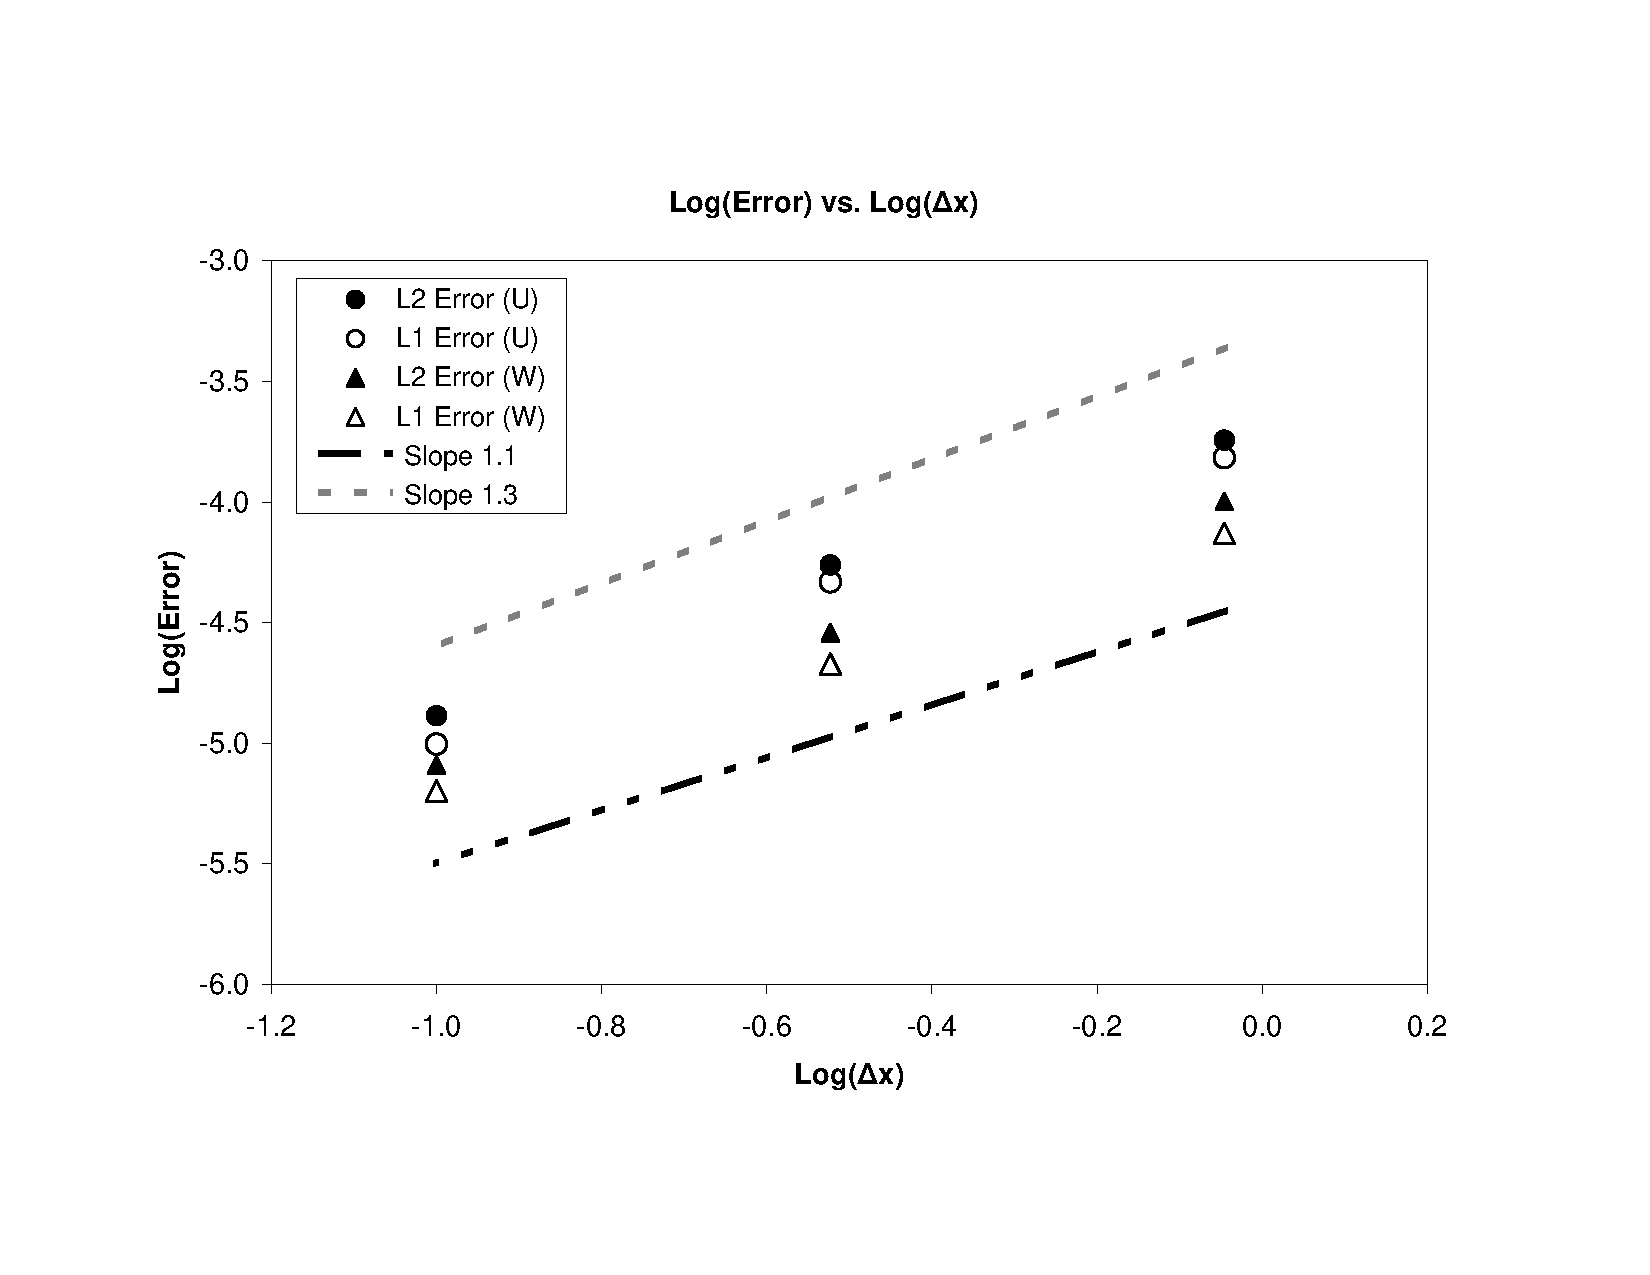
\includegraphics[width=5.5in]{../figures/GridConvTest/GridConvTest_dt0p01.pdf}
\label{fig:GridConvTest_dt0p01}
\vspace{-0.2in}
\caption{Grid Convergence Test. dt=0.01. 6 original points}
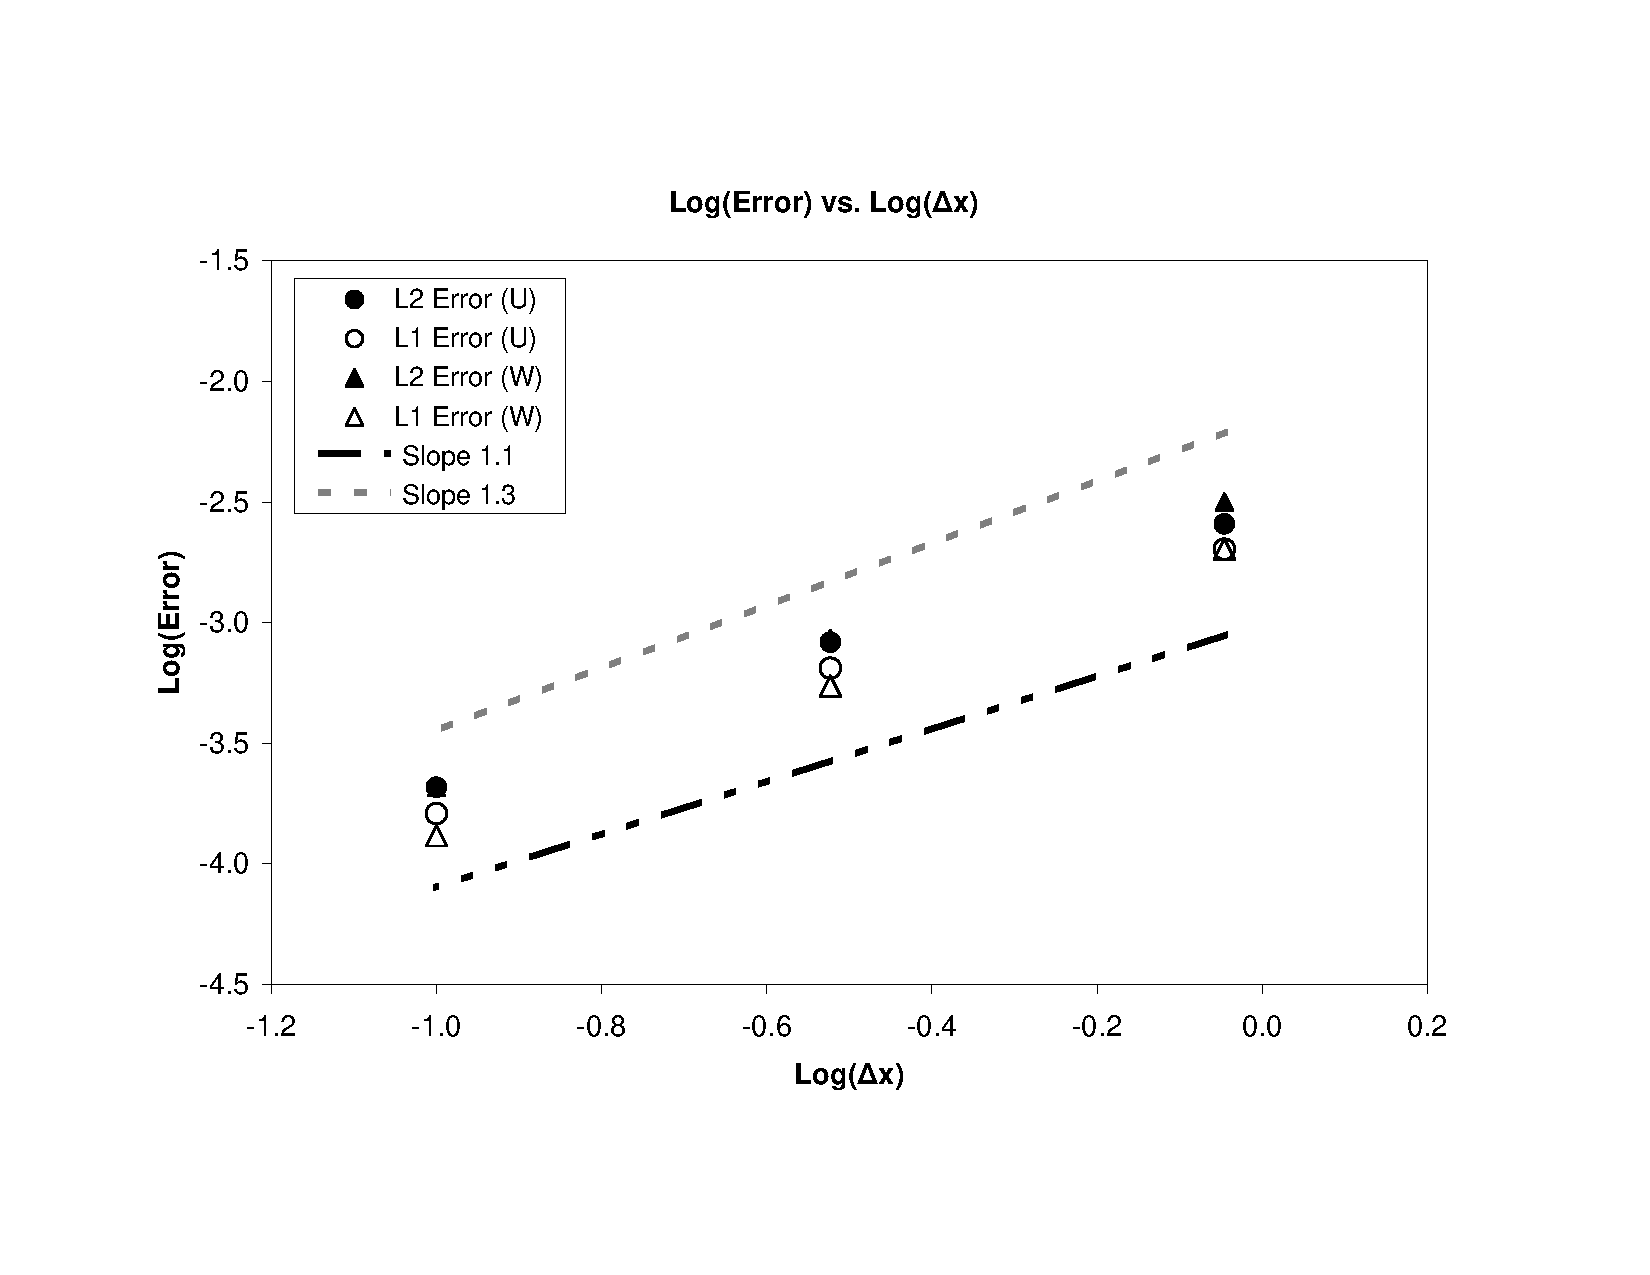
\includegraphics[width=5.5in]{../figures/GridConvTest/GridConvTest.pdf}
\label{fig:GridConvTest}
\vspace{-0.2in}
\caption{Grid Convergence Test. dt=0.2. 9 points}
\end{center}
\end{figure}
\end{comment}


\cp
